\documentclass[spanish, 10pt,a4paper]{article}
\usepackage[spanish]{babel}
\usepackage[utf8]{inputenc}
\usepackage{textcomp}
\usepackage{hyperref}
\usepackage[pdftex]{graphicx}
\usepackage{epsfig}
\usepackage{amsmath}
\usepackage{hyperref}
\usepackage{amssymb}
\usepackage{color}
\usepackage{graphics}
\usepackage{clrscode3e}
\usepackage{amsthm}
\usepackage{caratula}
\usepackage{fancyhdr,lastpage}
\usepackage[paper=a4paper, left=0.8cm, right=0.8cm, bottom=1.4cm, top=1.4cm]{geometry}
\usepackage[table]{xcolor} % color en las matrices
\usepackage[font=small,labelfont=bf]{caption} % caption de las figuras en letra mas chica que el texto
\usepackage[ruled,vlined,linesnumbered]{algorithm2e}
\usepackage{listings}
\usepackage{float}
\usepackage{amsfonts}
\usepackage{upgreek}
\usepackage{anysize} 
\usepackage[utf8]{inputenc}
\usepackage{babel}
\usepackage{hyperref}
\usepackage[pdftex]{graphicx}
\usepackage{amsfonts}
\usepackage{amsmath}
\usepackage{colortbl}
\usepackage{pdfpages}
\usepackage{titlesec}
\usepackage[margin=1cm]{subcaption}


\color{black}

%%%PAGE LAYOUT%%%
\topmargin = -1.2cm
\voffset = 0cm
\hoffset = 0em
\textwidth = 48em
\textheight = 164 ex
\oddsidemargin = 0.5 em
\parindent = 1 em
\parskip = 3 pt
\footskip = 7ex
\headheight = 20pt
\pagestyle{fancy}
\lhead{Redes Neuronales - 2017 C1 - Trabajo Pr\'actico 2} % cambia la parte izquierda del encabezado
\renewcommand{\sectionmark}[1]{\markboth{#1}{}} % cambia la parte derecha del encabezado
\rfoot{\thepage}
\cfoot{}
\numberwithin{equation}{section} %sets equation numbers <chapter>.<section>.<subsection>.<index>

%Lo siguiente controla el ancho de las figuras (principalmente para el texto de los captions)
%\newcommand{\figurewidth}{.9\textwidth}
\newcommand{\figurewidth}{1\textwidth}

\newcommand{\tuple}[1]{\ensuremath{\left \langle #1 \right \rangle }}
\newcommand{\Ode}[1]{\small{$\mathcal{O}(#1)$}}
\newtheorem{teorema}{Teorema}[section]

\def\changemargin#1#2{\list{}{\rightmargin#2\leftmargin#1}\item[]}
\let\endchangemargin=\endlist 


%El siguiente paquete permite escribir la caratula facilmente
\hypersetup{
  pdftitle={ TLeng TP },
  colorlinks,
  citecolor=black,
  filecolor=black,
  linkcolor=black,
  urlcolor=black 
}

\materia{Redes Neuronales}

\titulo{Trabajo Práctico 2}

\subtitulo{Aprendizaje No Supervisado}

\grupo{}

\integrante{Bonet, Felipe}{}{fpbonet@gmail.com}
\integrante{Martínez, Federico}{}{fedomartinez@hotmail.com}
\integrante{Avendano, Demian}{}{demian.avendano@gmail.com}
 
\begin{document}
{ \oddsidemargin = 2em
	\headheight = -20pt
	\maketitle
}
	\tableofcontents
	\newpage
	
\section{Introducción}


\textit{En este documento se realizan las actividades propuestas en el TP 2, actividades relacionadas con la implementación de dos problemas de clasificación.
El primero de ellos relacionado a la reducción de dimensionalidad de un set de datos. El segundo, confección de mapas autoorganizados. El objetivo del
trabajo es desarrollar redes neuronales que propongan soluciones a ambos.}

\subsection{Introducción al problema}
Las redes neuronales son modelos computacionales, en los que se intenta emular el funcionamiento fisiológico de un conjunto de neuronas biológicas, interconectadas, con el fin de lograr predicciones a partir de un conjunto de datos similares, presentados previamente. Para ello se modelan, en cada unidad de procesamiento, características que tienen que ver con las condiciones de propagación de señales electroquímicas. Estas condiciones se describen y modelan a partir de observaciones de sobre cómo es transmitida información entre una neurona y otra (o sobre si), y sobre como se encuentran interconectadas.

La suma de las interacciones entre estas unidades modeladas en una topología dada, genera propiedades emergentes que permiten  resolver cierto tipos de  problemas (en el caso de este trabajo, problemas de clasificación de elementos). 
Para intentar resolver estos problemas utilizando redes neuronales, es necesario recurrir a diversas técnicas para el ajuste de las variables de la red, y en muchos casos se requiere un paso de preprocesamiento de los datos.

En ambos casos utilizamos redes de aprendizaje no supervisado. Para el primer problema, la técnica utilizada fue aprendizaje hebbiano. Para el segundo, redes autoorganizadas. 

Los valores de entrada fueron clasificaciones de empresas brasileras en base a 850 atributos, originalmente derivados de una descripción en palabras. La idea final del trabajo fue poder predecir estas clasificaciones con redes de aprendizaje no supervisado y poder entrenarlas para lograrlo de la manera más precisa posible.

\subsection{Entrega}
\subsection{Requerimientos}
\begin{itemize}
\item Intérprete python 2.7.
\item Librerías estandar, librería \textit{matplotlib} y \textit{numpy}.
\item Archivo CSV con uno de los dos formatos propuestos en el TP. 
\end{itemize}

\subsection{Modo de uso y opciones}
Para usar este programa, se deben ejecutar el archivo \textbf{script.py}, el cual contiene todas las opciones de ejecución. Para ello, tipear por consola :

\texttt{\$python script.py N args}

donde \texttt{N} es el número de ejercicio y \texttt{args} son los argumentos optativos. Es obligatorio proveer el número de ejercicio, ya que se parsean los inputs de forma distinta. A su vez, cambian los métodos de cálculo de eficacia de la red.\\

Las opciones disponibles son:

\subsubsection{Opciones}

% \textbf{-file}: Filepath del dataset que se desee utilizar para entrenar o predecir resultados. Si no se lo provee, por default el programa buscará el archivo $tp1_ej1_training.csv$ o $tp1_ej2_training.csv$ en la carpeta donde se esté ejecutando, dependiendo del número de ejercicio pasado anteriormente.

% \textbf{-ep}: Cantidad de épocas por default, 500.

% \textbf{-eta}: Tasa de aprendizaje, por default $\eta$ = 0.05

% \textbf{-capas}: Capas ocultas de la red, cada número separado por una coma representa una capa y cada magnitud de la capa representa la cantidad de neuronas de esa capa, por default = '10,10', o sea, dos capas de 10 neuronas cada una.

% \textbf{-tr}:  Cantidad en \% del total de datos utilizado para entrenar a la red, por default = 70.

% \textbf{-te}: Cantidad en \% del total de datos utilizado para testing, por default = 20

% \textbf{-val}: Cantidad en \% del total de datos utilizados como validación, por default = 10

% \textbf{-tambatch}: Tamaño del batch de aprendizaje a utilizar. Por default el valor es $1$, es decir entrenamiento estocástico.

% \textbf{-mo}: Magnitud del momentum a utilizar. Default es 0.

% \textbf{-fa}: Función de activación, puede ser \textit{tangente o logística}, por default es \textit{tangente}.

% \textbf{-dp}: Distribución de inicialización de pesos a utilizar, puede ser \textit{normal} o \textit{uniforme}, por default se usa \textit{normal}.

% \textbf{-rda}: Permite cargar una red entrenada desde un archivo con formato \textit{JSON}. Se debe proveer el filepath del archivo JSON. En caso de no proveer este parámetro, se generará una red nueva, entrenándola con el dataset seleccionado.

% \textbf{-rha}: Permite almacenar una red entrenada a un archivo con \textit{JSON}. Se debe proveer el filepath destino del archivo JSON.

% \textbf{-estop}: Utilizado para activar early stopping. El argumento es el treshold a considerar. Default = 0.

% \textbf{-adap}: Define si se utiliza o no parámetros adaptativos. Valores = 0 o 1. Default = 0.

\subsection{Archivos}
Para la resolución del trabajo, fue necesario desarrollar en primer lugar un parser de los datos de entrada. El código de las funciones de parsing esta en \textbf{script.py}. Allí se encuentran la inicialización del programa, junto con el parseo de los parámetros, su normalización y el llamado a las funciones y métodos de la red.\\

El código propiamente de la red se encuentra en \textbf{network.py}. Allí están todas las funciones de los procesos de inicialización, computación de pesos y resultados.\\

% El parsing y definición de parámetros está en \textbf{parameters.py}. Las funciones encargadas de la normalización de los datos se encuentra en \textbf{normalizer.py}. Las funciones encargadas de codificar y decodificar redes entrenadas en formato json se hallan en \textbf{encoder.py}\\

% \subsection{Otros scripts}

% Se proveen a su vez los scripts utilizados para los experimentos, en caso de desear ejecutarlos. En la sección Resultados comentaremos donde se encuentra el código utilizado para cada uno.

	\newpage
	\section{Resultados}
En esta sección incluiremos los resultados de la experimentación que realizamos con las redes desarrolladas.\\

La idea general de los experimentos es intentar medir la performance
de cada red observando, en el primer problema, la distribución espacial de los clusters de empresas y en el segundo, la calidad 
del mapa generado.\\

Presentamos en primer lugar los resultados obtenidos del problema de reducción de dimensiones.

\subsection{Ejercicio 1 - Reducción de dimensiones}

Para el primer ejercicio, los experimentos consistieron en variar la cantidad de épocas, la regla de aprendizaje y la cantidad de dimensiones de salida. Intentamos variar estos factores y observar diferencias en los gráficos 3D generados en base a las nuevas dimensiones.

Comenzamos realizando clasificaciones con 100 épocas. Al obtener resultados imprecisos subimos la cantidad a 200. Allí observamos una clasificación mejor, más marcada la separación geométrica entre los distintos clusters.

Luego comparamos los resultados obtenidos entre las distintas reglas. Repetimos las ejecuciones variando la regla entre Oja y Sanger para comprobar su eficacia.

Por último, decidimos cambiar la cantidad de dimensiones de sálida, esperando una mejora en las clasificaciones. 

\subsubsection{Regla de Oja - variando número de épocas}
En los primeros experimentos, fuimos probando la calidad de la clasificación utilizando solamente 100 épocas. La decisión se basó en un tema de performance de la red. Cada ejecución tenía una considerable demora, por lo que empezamos probando con pocas épocas. Mostramos los primeros resultados que obtuvimos, utilizando la regla de Oja:

\begin{figure}[!htbp]
\centering
\begin{subfigure}{.5\textwidth}
  \centering
  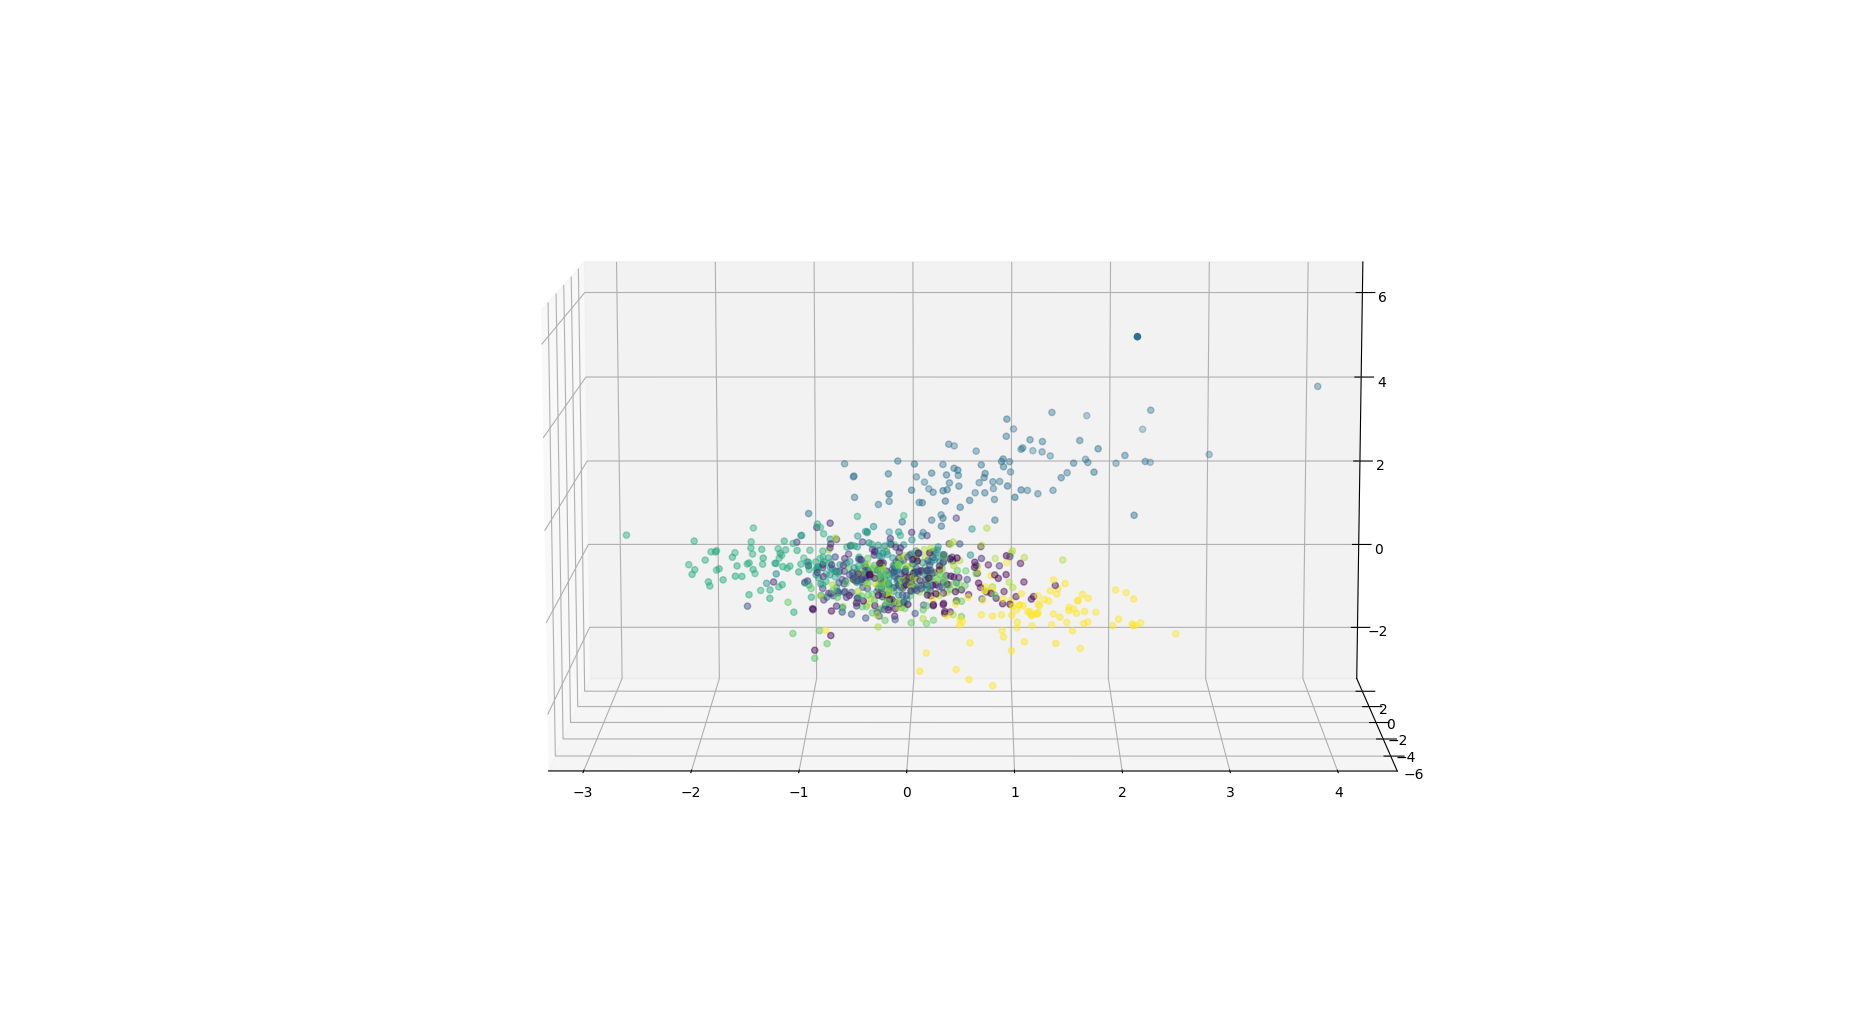
\includegraphics[width=1\linewidth, scale=1]{../img/ej1/oja/oja_3salida_100ep_train_2.png}
  \caption{Oja - 3 dimensiones - 100 épocas}
  \label{fig:sub1}
\end{subfigure}%
\begin{subfigure}{.5\textwidth}
  \centering
  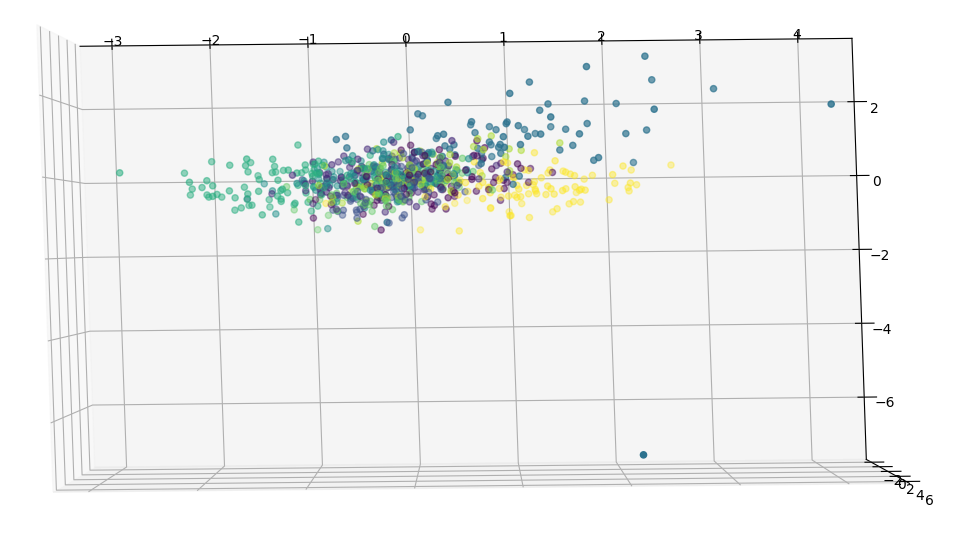
\includegraphics[width=1\linewidth, scale=1]{../img/ej1/oja/oja_3salida_100ep_train_3.png}
  \caption{Oja - 3 dimensiones - 100 épocas}
  \label{fig:sub2}
\end{subfigure}
\end{figure}

\newpage

\begin{figure}[h]
  \begin{center}
    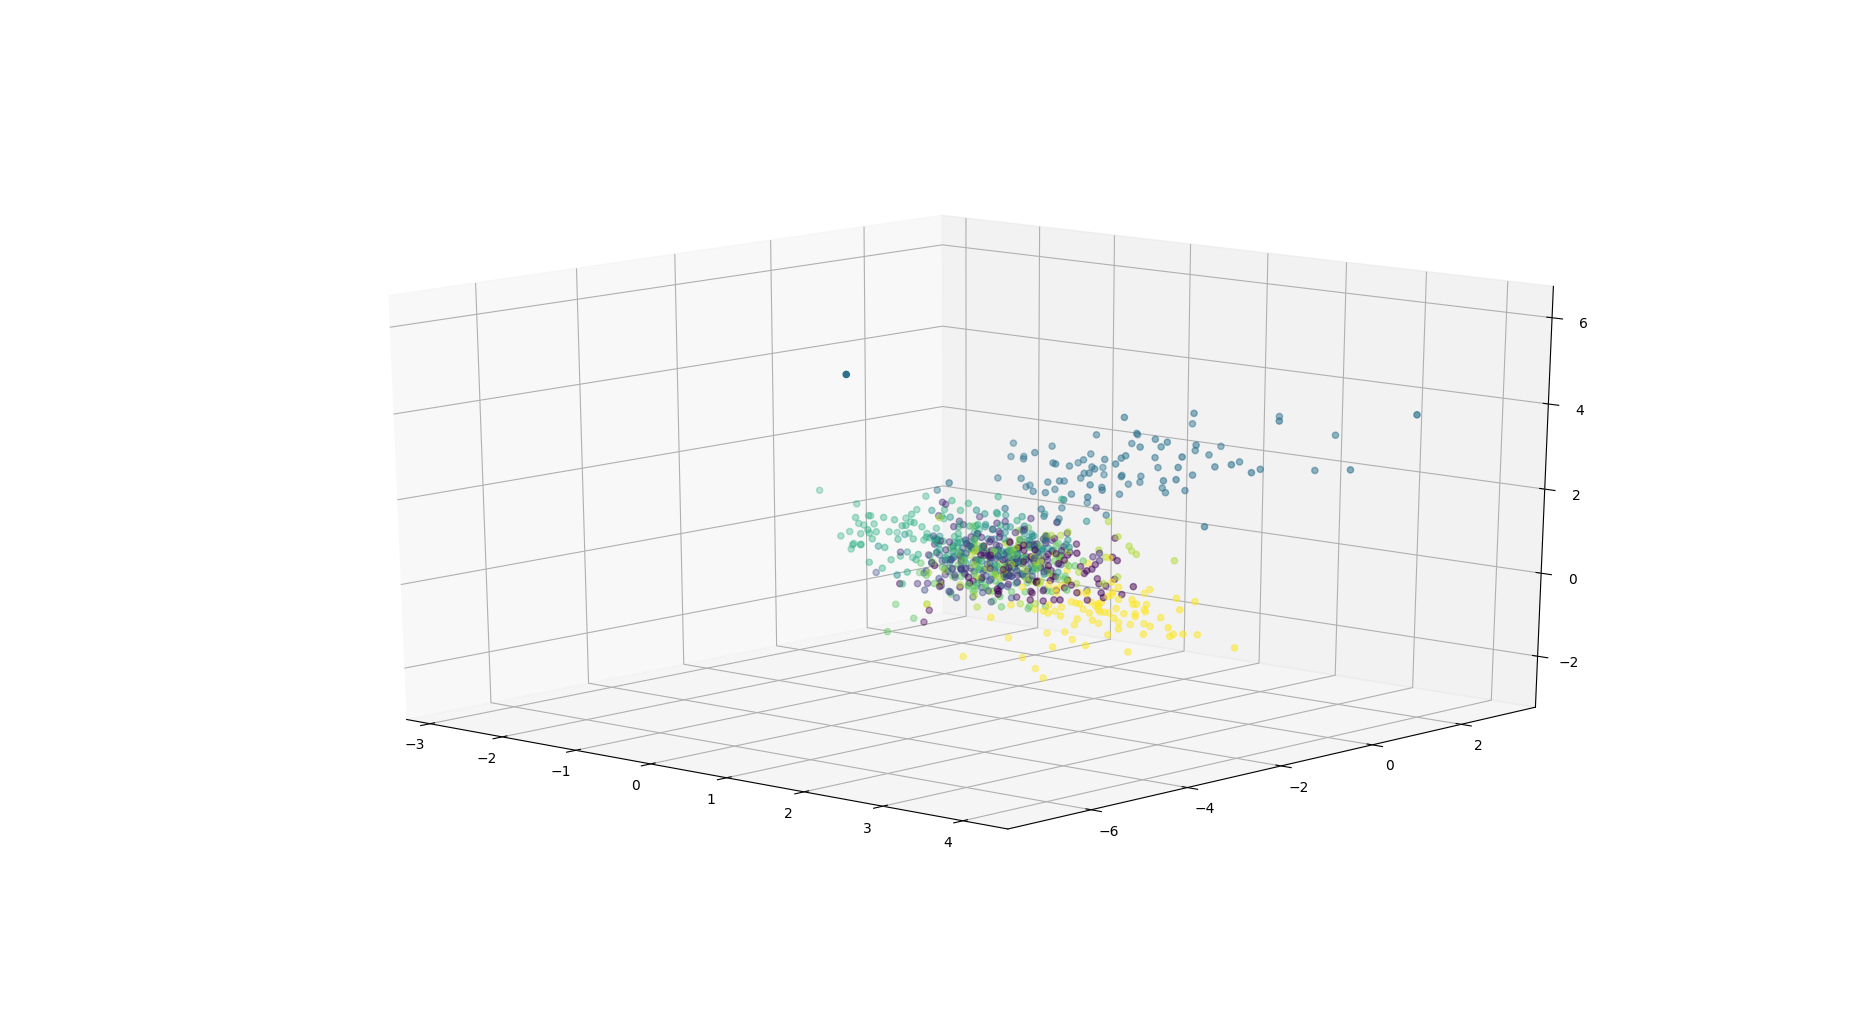
\includegraphics[scale=0.45]{../img/ej1/oja/oja_3salida_100ep_train.png}
  \caption{Oja - 3 dimensiones - 100 épocas - Datos Entrenamiento}
  \end{center}
\end{figure}

Éstos son los gráficos de las ejecuciones utilizando regla de Oja, con 100 épocas. Notamos que se están comenzando a formar
clusters de clasificación con distintos colores, pero que también hay mucho solapamiento en la parte central de cada vista.\\

Luego de esta etapa de entrenamiento, procesamos los datos de validación:

\begin{figure}[!htbp]
\centering
\begin{subfigure}{.5\textwidth}
  \centering
  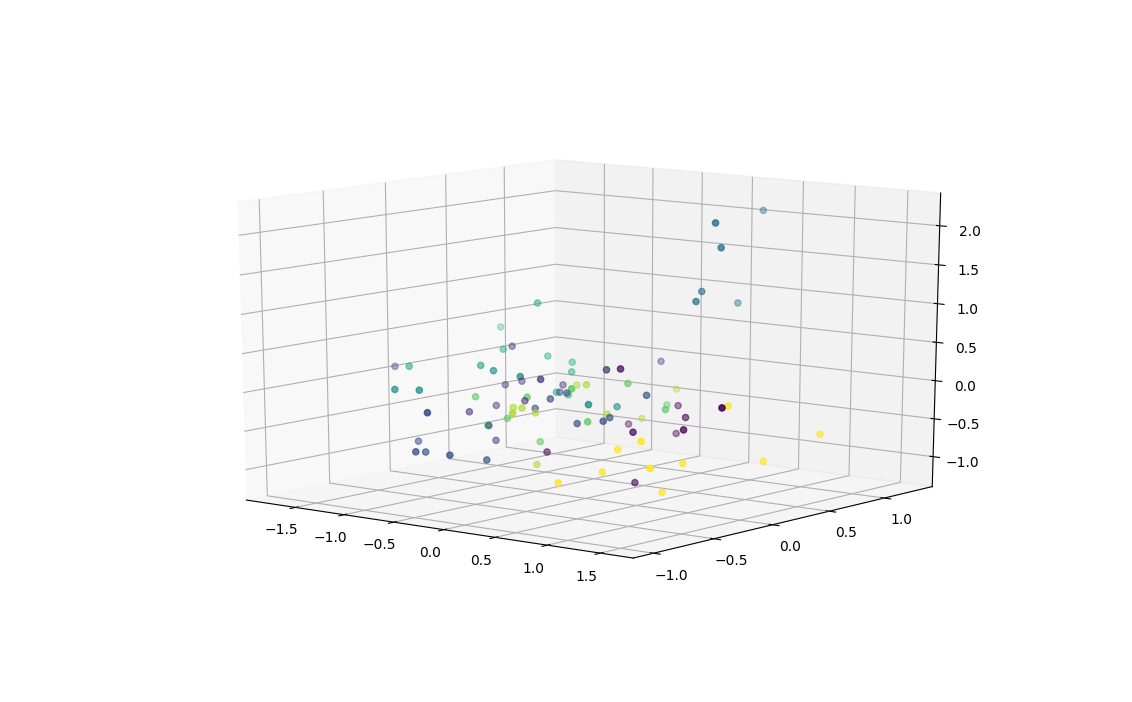
\includegraphics[width=1\linewidth, scale=1]{../img/ej1/oja/oja_3salida_100ep_validation.png}
  \caption{Oja - 3 dimensiones - 100 épocas}
  \label{fig:sub1}
\end{subfigure}%
\begin{subfigure}{.5\textwidth}
  \centering
  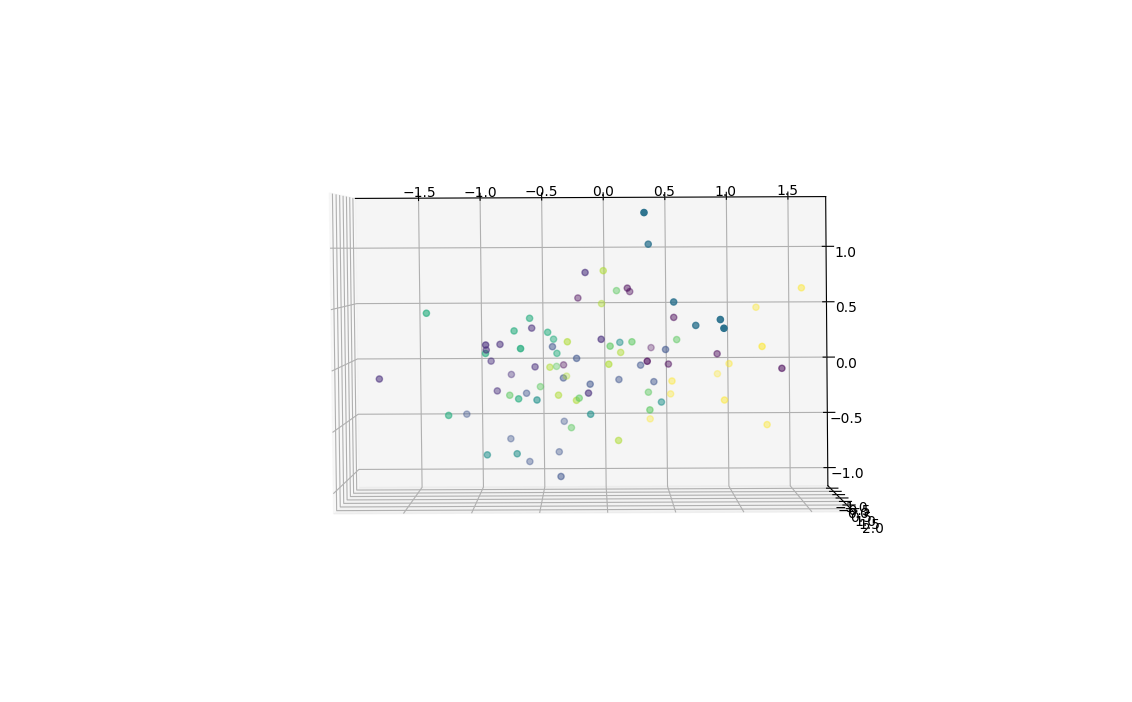
\includegraphics[width=1\linewidth, scale=1]{../img/ej1/oja/oja_3salida_100ep_validation_3.png}
  \caption{Oja - 3 dimensiones - 100 épocas}
  \label{fig:sub2}
\end{subfigure}
\end{figure}

\begin{figure}[h]
  \begin{center}
    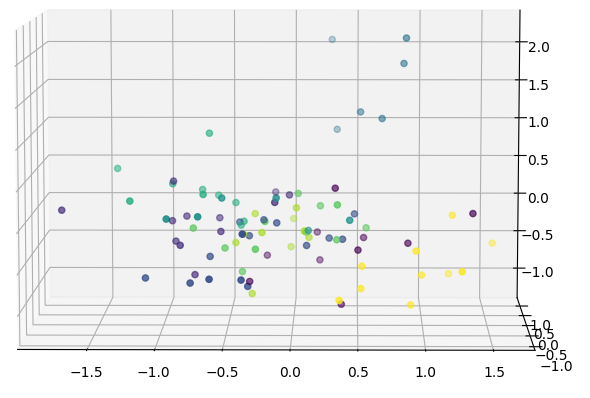
\includegraphics[scale=0.65]{../img/ej1/oja/oja_3salida_100ep_validation_2.png}
  \caption{Oja - 3 dimensiones - 100 épocas - Datos Validación}
  \end{center}
\end{figure}

\newpage

Para los datos de validación vemos una dispersión muy grande. Se notan algunos puntos del mismo color agrupados levemente cerca, pero lejos
de formar una división clara.\\

Luego de obtener estos resultados, menos precisos de lo que esperábamos, decidimos intentar probar subiendo número de épocas. Observemos a continuación las mismas ejecuciones, pero subiendo el número de épocas a 200:

\begin{figure}[!htbp]
\centering
\begin{subfigure}{.5\textwidth}
  \centering
  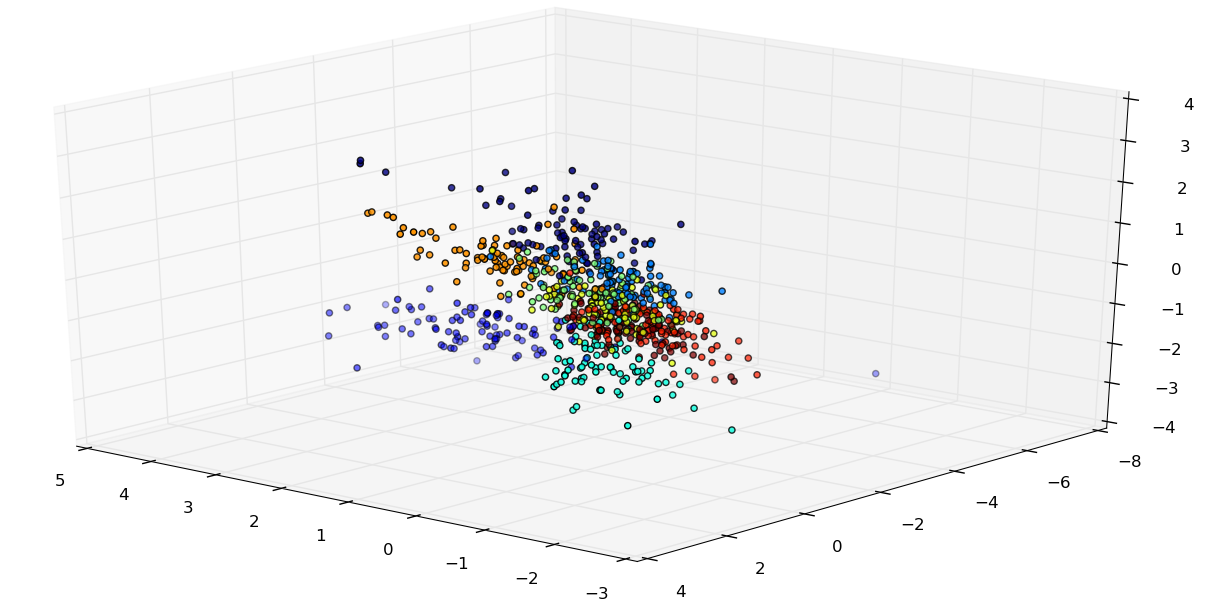
\includegraphics[width=1\linewidth, scale=1]{../img/ej1/oja/oja_3salida_200ep_train.png}
  \caption{Oja - 3 dimensiones - 200 épocas}
  \label{fig:sub1}
\end{subfigure}%
\begin{subfigure}{.5\textwidth}
  \centering
  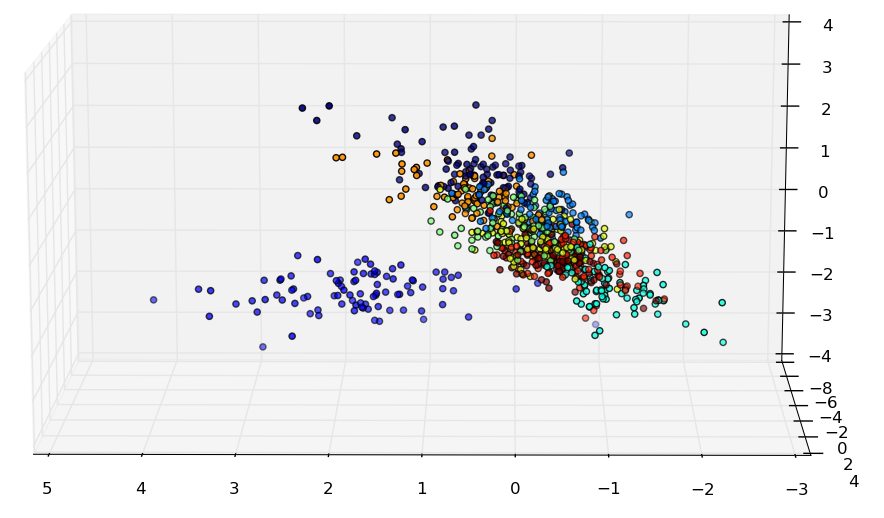
\includegraphics[width=1\linewidth, scale=1]{../img/ej1/oja/oja_3salida_200ep_train_2.png}
  \caption{Oja - 3 dimensiones - 200 épocas}
  \label{fig:sub2}
\end{subfigure}
\end{figure}
\begin{figure}[!htbp]
\centering
\begin{subfigure}{.5\textwidth}
  \centering
  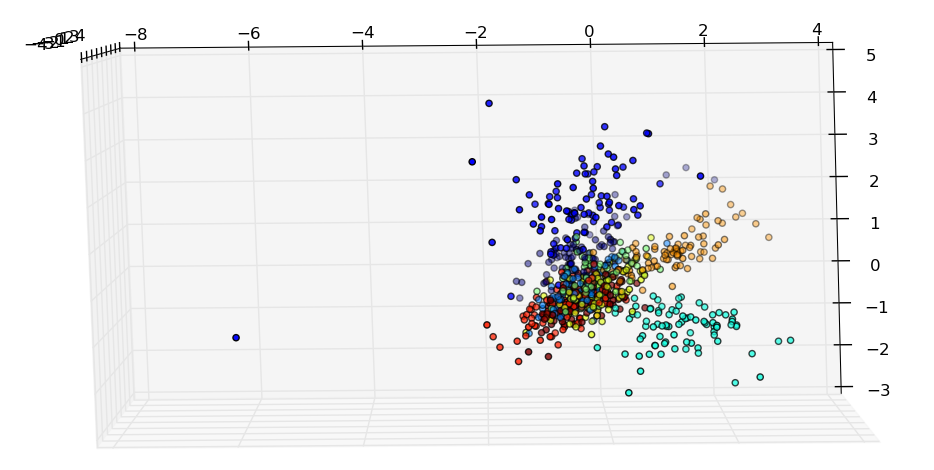
\includegraphics[width=1\linewidth, scale=1]{../img/ej1/oja/oja_3salida_200ep_train_3.png}
  \caption{Oja - 3 dimensiones - 200 épocas}
  \label{fig:sub3}
\end{subfigure}%
\begin{subfigure}{.5\textwidth}
  \centering
  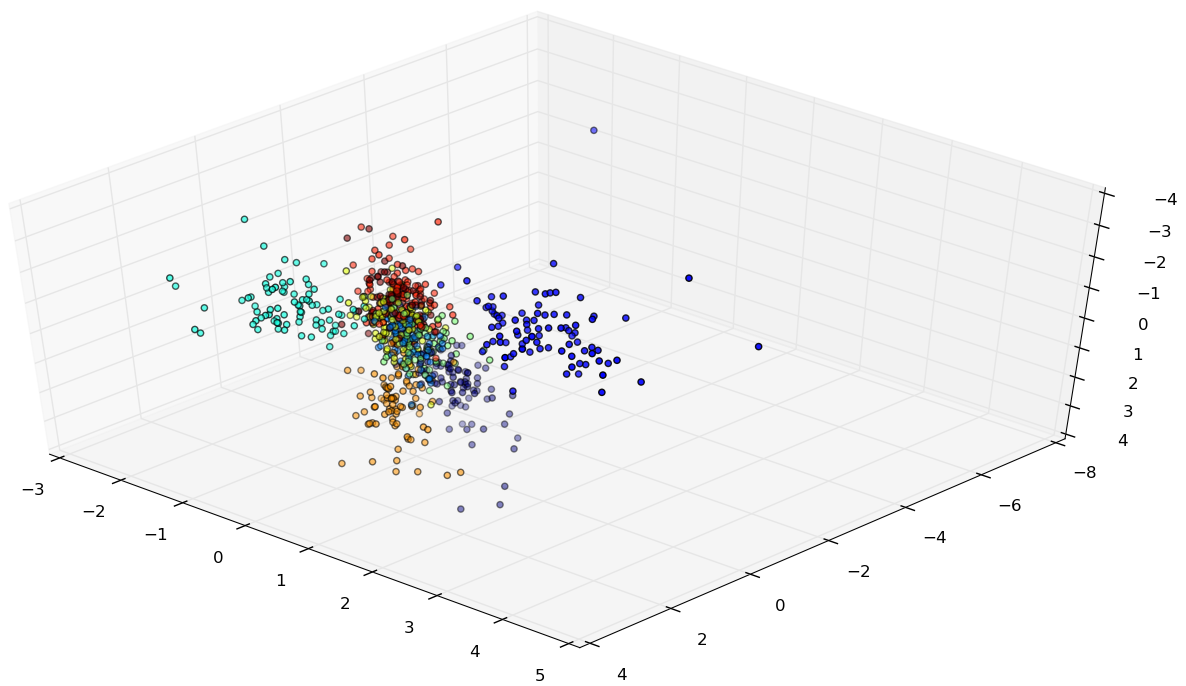
\includegraphics[width=1\linewidth, scale=1]{../img/ej1/oja/oja_3salida_200ep_train_4.png}
  \caption{Oja - 3 dimensiones - 200 épocas}
  \label{fig:sub4}
\end{subfigure}
\end{figure}

En los datos de entrenamiento se observa que con 200 épocas se empiezan a notar más visiblemente
los clusters de datos. Se observa una leve mejora en la clasificación con respecto a la versión de 100 épocas.

Podemos ver de todas formas que algunas de las categorías se encuentran mezcladas entre sí mientras otras están más claramente divididas.

A continuación los datos de validation.

\begin{figure}[!htbp]
\centering
\begin{subfigure}{.5\textwidth}
  \centering
  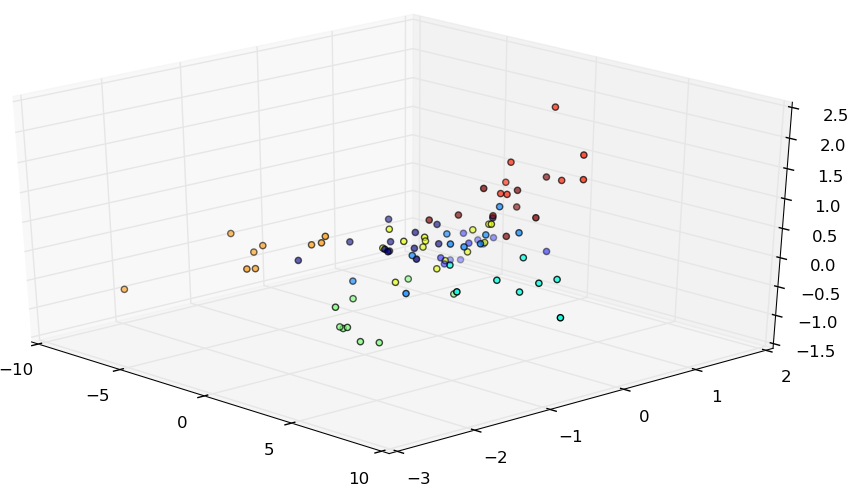
\includegraphics[width=1\linewidth, scale=1]{../img/ej1/oja/oja_3salida_200ep_validation.png}
  \caption{Oja - 3 dimensiones - 200 épocas}
  \label{fig:sub1}
\end{subfigure}%
\begin{subfigure}{.5\textwidth}
  \centering
  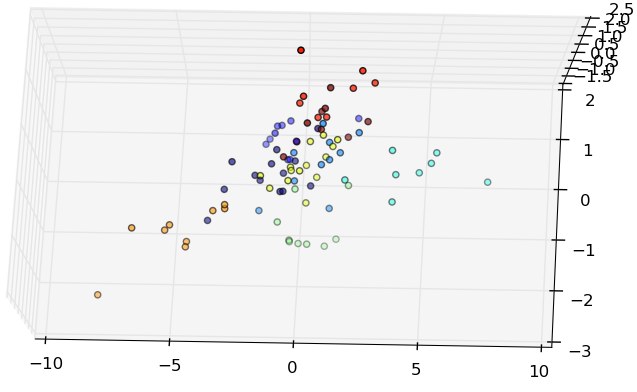
\includegraphics[width=1\linewidth, scale=1]{../img/ej1/oja/oja_3salida_200ep_validation_3.png}
  \caption{Oja - 3 dimensiones - 200 épocas}
  \label{fig:sub2}
\end{subfigure}
\end{figure}

\begin{figure}[h]
  \begin{center}
    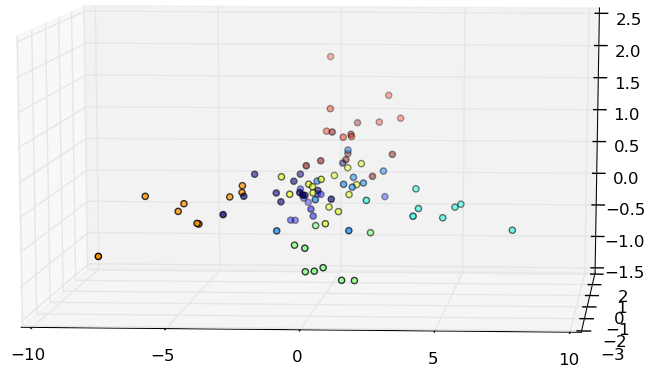
\includegraphics[scale=0.65]{../img/ej1/oja/oja_3salida_200ep_validation_2.png}
  \caption{Oja - 3 dimensiones - 200 épocas - Datos Validación}
  \end{center}
\end{figure}

En esta segunda tanda de gráficos se observa una mejora leve también para los datos de validación. Podemos ver que la mayoría de las marcas del mismo color están aproximadamente cercanas entre sí.

\subsubsection{Regla de Sanger - variando número de épocas}
Repetimos en este caso el experimento anterior utilizando ahora la regla de Sanger. Intentaremos comprobar si con esta nueva regla de aprendizaje
se obtienen mejores resultados variando el número de épocas.

En primer lugar, resultados con 100 épocas:

\newpage

\begin{figure}[!htbp]
\centering
\begin{subfigure}{.5\textwidth}
  \centering
  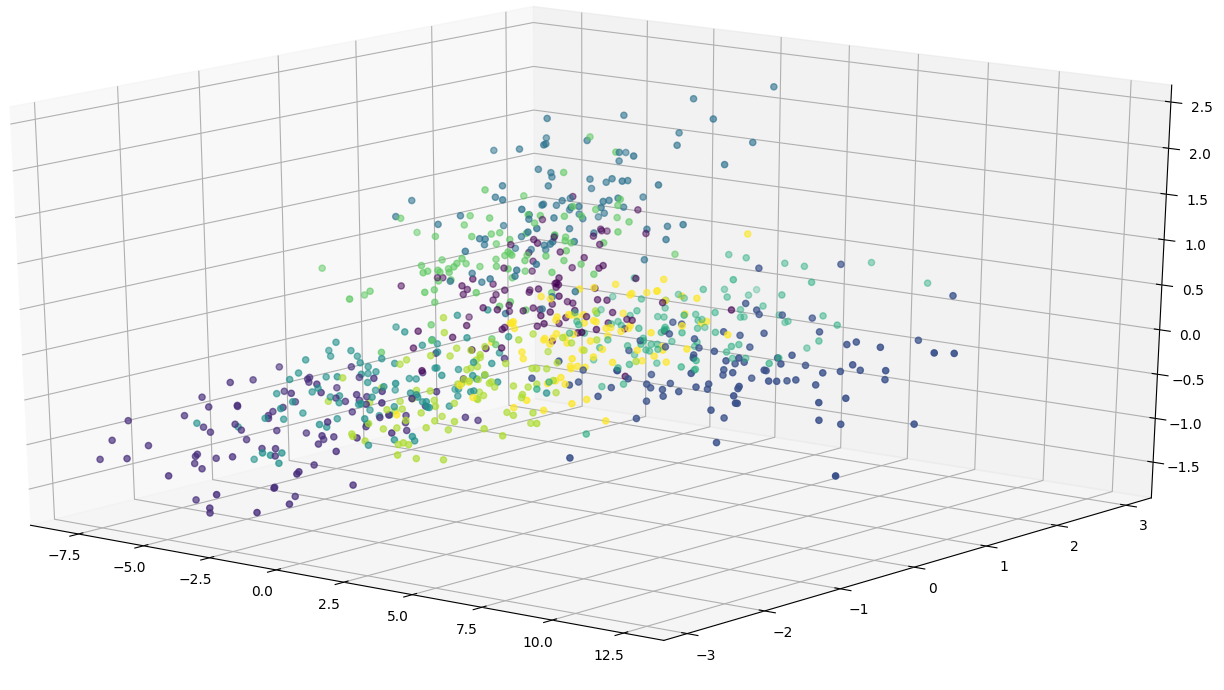
\includegraphics[width=1\linewidth, scale=1]{../img/ej1/sanger/sanger_3salida_100ep_train.png}
  \caption{Sanger - 3 dimensiones - 100 épocas}
  \label{fig:sub1}
\end{subfigure}%
\begin{subfigure}{.5\textwidth}
  \centering
  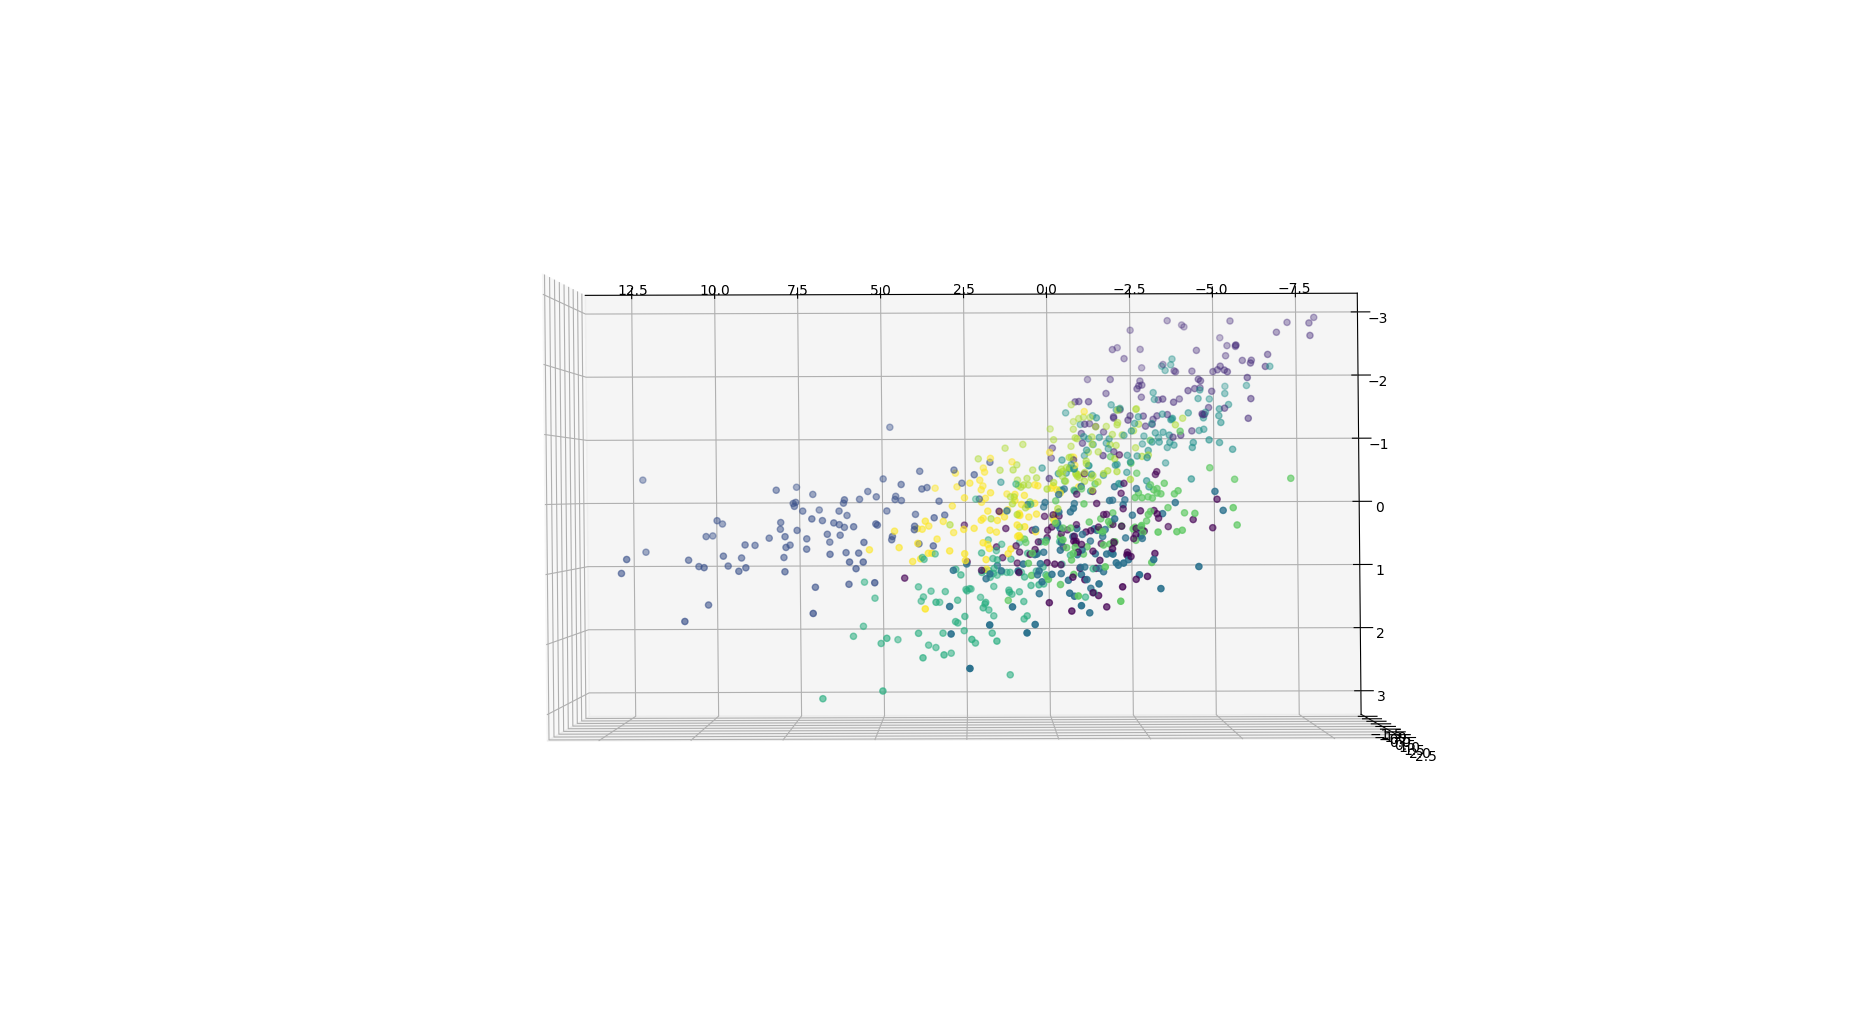
\includegraphics[width=1\linewidth, scale=1]{../img/ej1/sanger/sanger_3salida_100ep_train_3.png}
  \caption{Sanger - 3 dimensiones - 100 épocas}
  \label{fig:sub2}
\end{subfigure}
\end{figure}

\begin{figure}[h]
  \begin{center}
    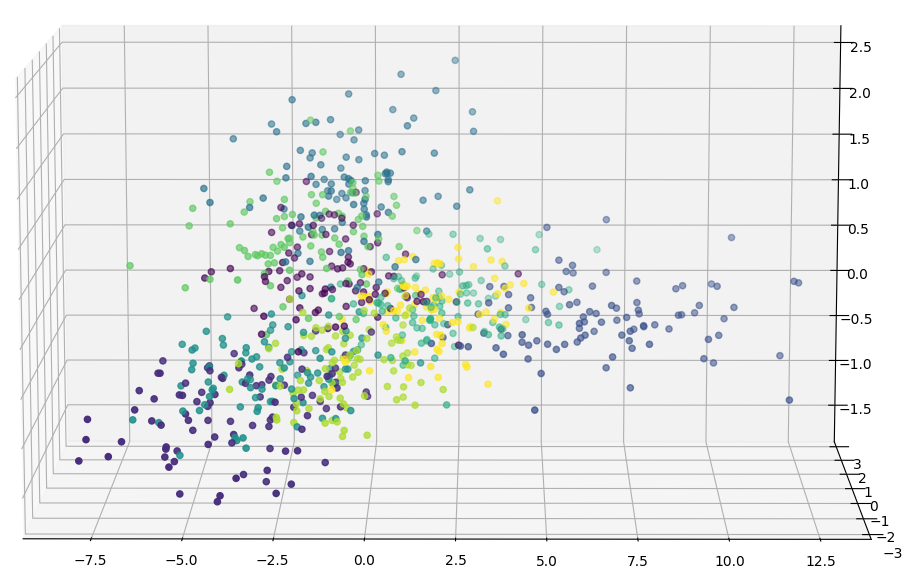
\includegraphics[scale=0.45]{../img/ej1/sanger/sanger_3salida_100ep_train_2.png}
  \caption{Sanger - 3 dimensiones - 100 épocas - Datos Entrenamiento}
  \end{center}
\end{figure}

Éstos son los resultados de las ejecuciones utilizando regla de Sanger, con 100 épocas. Notamos un gran nivel de dispersión y 
solapamiento entre las categorías. No tienen la calidad que esperábamos.

Luego de esta etapa de entrenamiento, procesamos los datos de validación. No obtuvimos buenos resultados, las marcas están 
medianamente agrupadas pero con alto nivel de disgregación.

\begin{figure}[!htbp]
\centering
\begin{subfigure}{.5\textwidth}
  \centering
  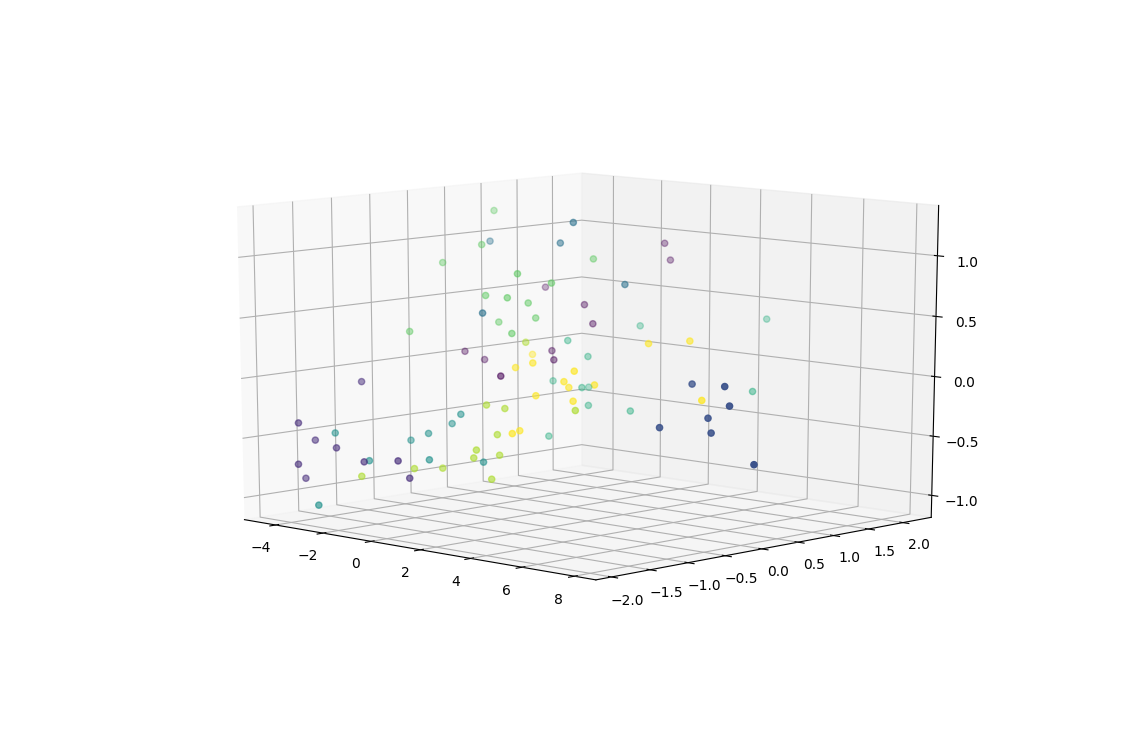
\includegraphics[width=1\linewidth, scale=1]{../img/ej1/sanger/sanger_3salida_100ep_validation.png}
  \caption{Sanger - 3 dimensiones - 100 épocas}
  \label{fig:sub1}
\end{subfigure}%
\begin{subfigure}{.5\textwidth}
  \centering
  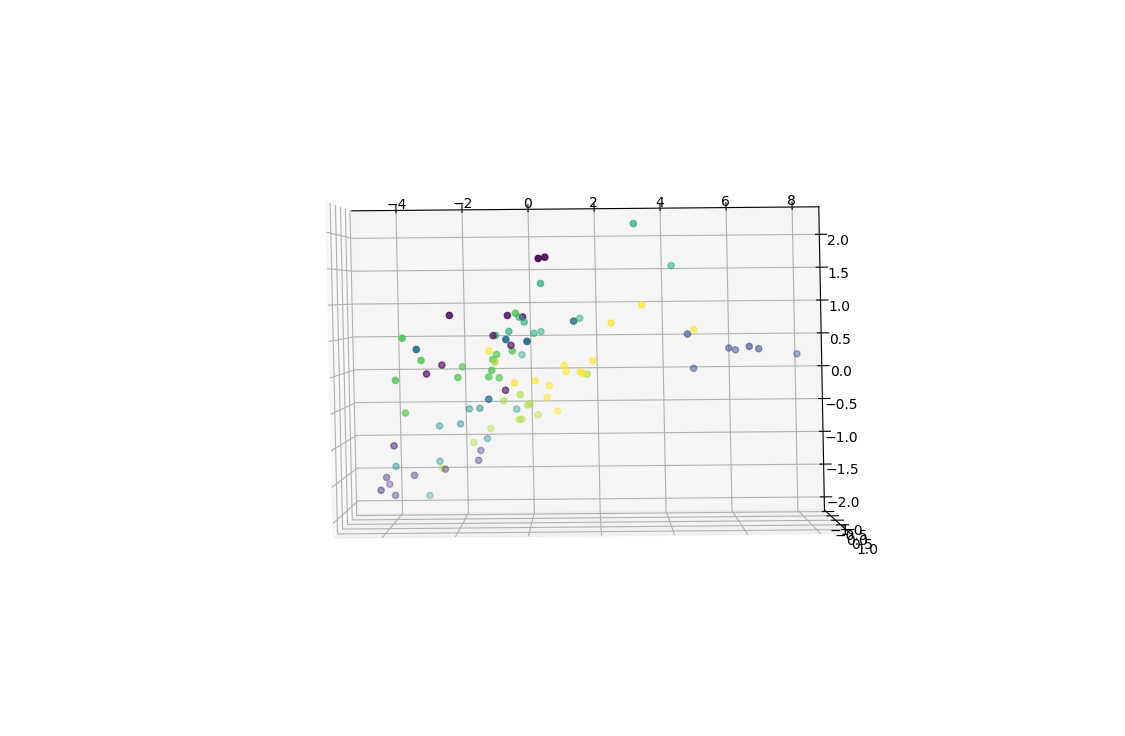
\includegraphics[width=1\linewidth, scale=1]{../img/ej1/sanger/sanger_3salida_100ep_validation_3.png}
  \caption{Sanger - 3 dimensiones - 100 épocas}
  \label{fig:sub2}
\end{subfigure}
\end{figure}

\begin{figure}[h]
  \begin{center}
    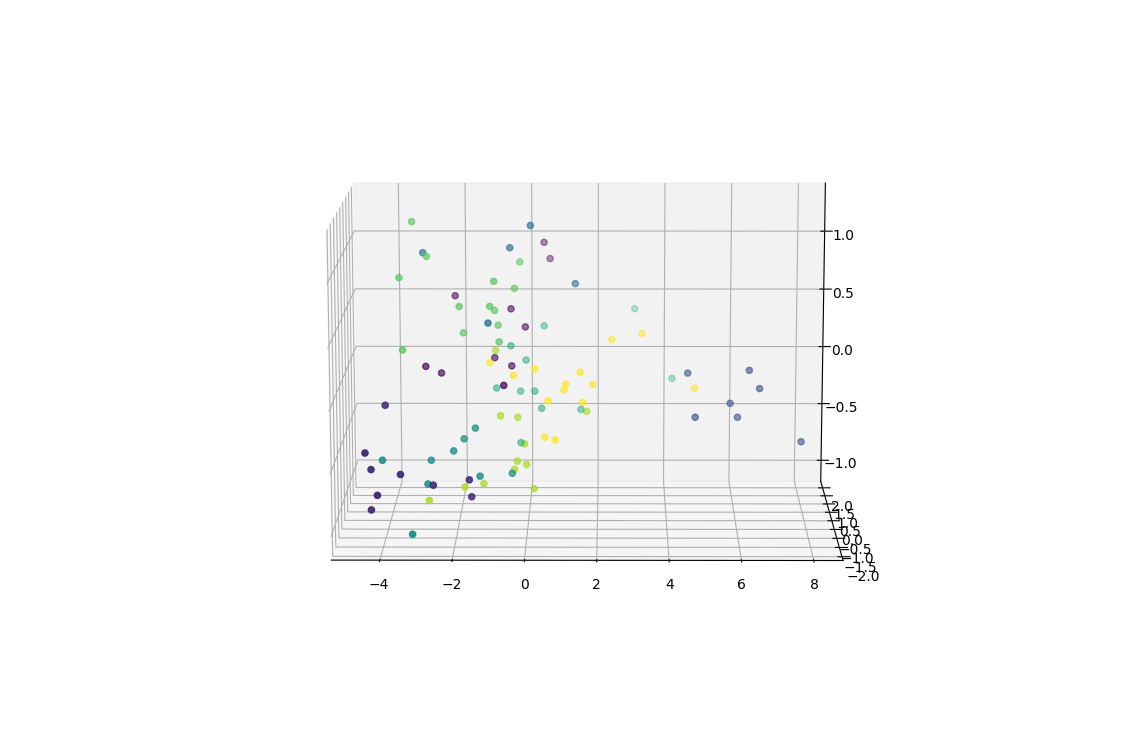
\includegraphics[scale=0.65]{../img/ej1/sanger/sanger_3salida_100ep_validation_2.png}
  \caption{Sanger - 3 dimensiones - 100 épocas - Datos Validación}
  \end{center}
\end{figure}

\newpage

Para los datos de validación vemos, que al igual que en Oja, los resultados con solo 100 épocas no son los mejores.

Observemos a continuación las mismas ejecuciones, pero subiendo el número de épocas a 200:

\begin{figure}[h]
  \begin{center}
    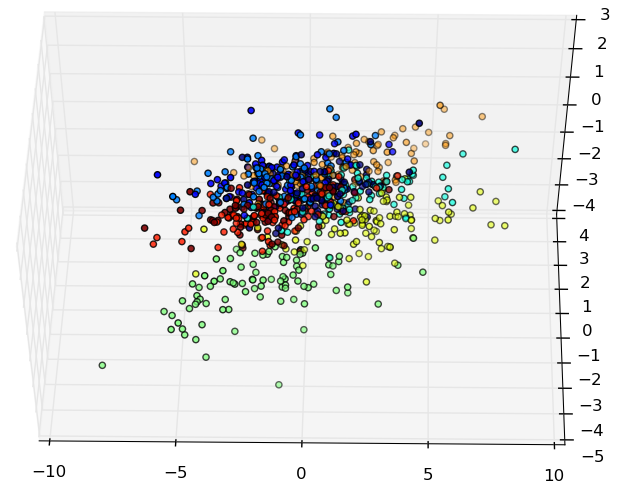
\includegraphics[scale=0.75]{../img/ej1/sanger/sanger_3salida_200ep_train_2.png}
  \caption{Sanger - 3 dimensiones - 200 épocas - Datos Validación}
  \end{center}
\end{figure}

\newpage

\begin{figure}[!htbp]
\centering
\begin{subfigure}{.5\textwidth}
  \centering
  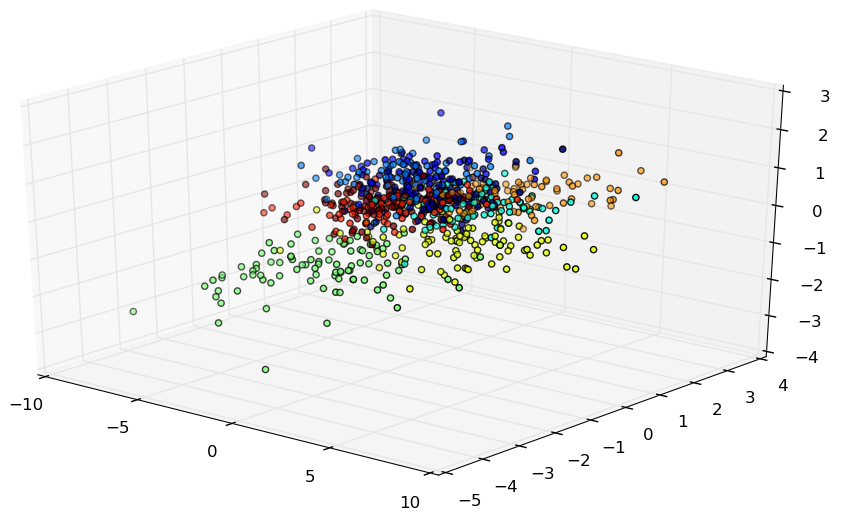
\includegraphics[width=1\linewidth, scale=1]{../img/ej1/sanger/sanger_3salida_200ep_train.png}
  \caption{Sanger - 3 dimensiones - 200 épocas}
  \label{fig:sub1}
\end{subfigure}%
\begin{subfigure}{.5\textwidth}
  \centering
  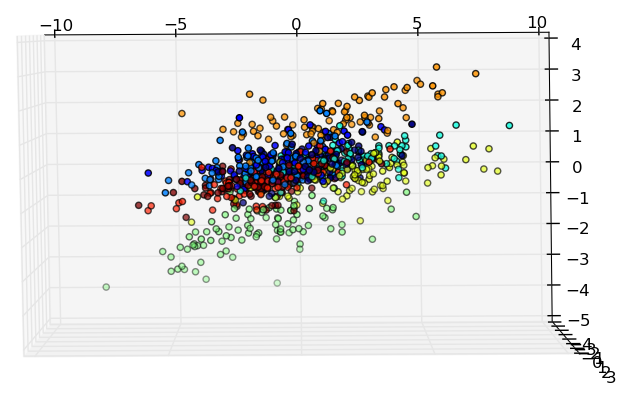
\includegraphics[width=1\linewidth, scale=1]{../img/ej1/sanger/sanger_3salida_200ep_train_3.png}
  \caption{Sanger - 3 dimensiones - 200 épocas}
  \label{fig:sub2}
\end{subfigure}
\end{figure}

En los datos de entrenamiento observamos que con 200 épocas los clusters de datos se encuentran un poco más definidos. 
Se observa una notable mejora en la clasificación con respecto a la versión anterior de 100 épocas.

Podemos ver de todas formas que algunas de las categorías presentan alto nivel de solapamiento.

A continuación los datos de validation.

\begin{figure}[!htbp]
\centering
\begin{subfigure}{.5\textwidth}
  \centering
  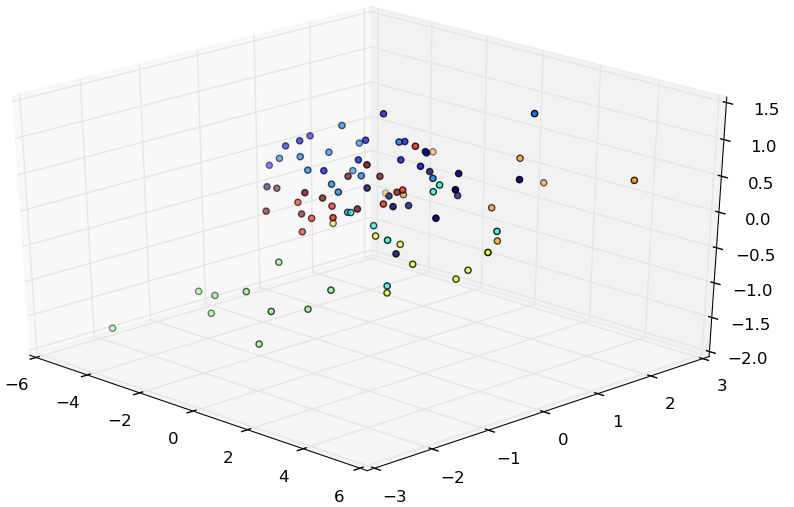
\includegraphics[width=1\linewidth, scale=1]{../img/ej1/sanger/sanger_3salida_200ep_validation.png}
  \caption{Sanger - 3 dimensiones - 200 épocas}
  \label{fig:sub1}
\end{subfigure}%
\begin{subfigure}{.5\textwidth}
  \centering
  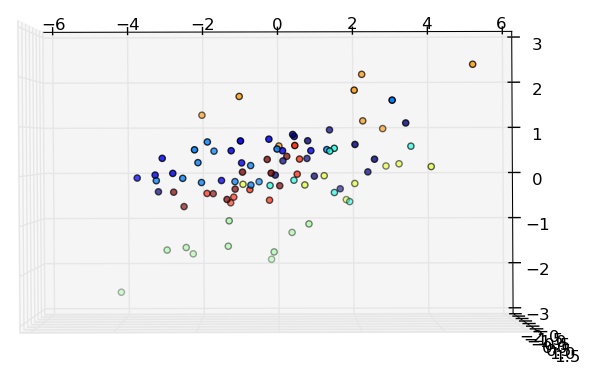
\includegraphics[width=1\linewidth, scale=1]{../img/ej1/sanger/sanger_3salida_200ep_validation_3.png}
  \caption{Sanger - 3 dimensiones - 200 épocas}
  \label{fig:sub2}
\end{subfigure}
\end{figure}

\begin{figure}[h]
  \begin{center}
    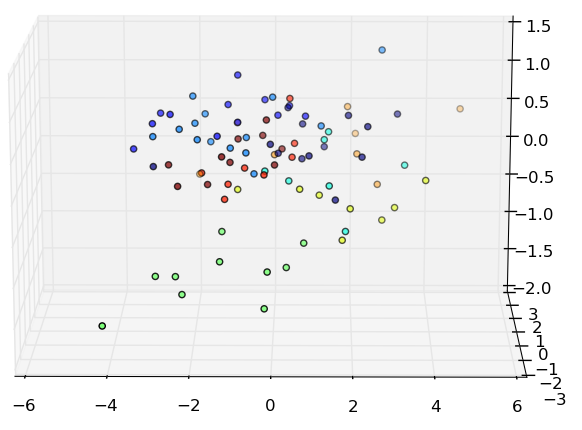
\includegraphics[scale=0.4]{../img/ej1/sanger/sanger_3salida_200ep_validation_2.png}
  \caption{Sanger - 3 dimensiones - 200 épocas - Datos Validación}
  \end{center}
\end{figure}

En esta segunda tanda de gráficos se observa una mejora leve también para los datos de validación. Podemos ver que la mayoría de las marcas del mismo color están aproximadamente cercanas entre sí.

Debido a la lenta performance de las pruebas con la red, continuar aumentando la cantidad de épocas se volvió inviable. De todas formas hicimos una prueba preliminar con 500 épocas para explorar la posibilidad de obtener mejores resultados. Éstos no fueron mejores que los presentados aquí con 200, por lo tanto no continuamos dicho experimento y nos quedamos con las 200.
\newpage
\subsubsection{Regla de Oja - Variando número de dimensiones}

Debido a los resultados obtenidos, intentamos buscar una forma de mejorar la precisión de la clasificación. Por sugerencia docente, decidimos intentar aumentar la dimensionalidad de la salida. En lugar de reducir a 3 dimensiones como pide el enunciado, subimos la cantidad a 9 dimensiones, esperando obtener mejores resultados. \\
Debido a la imposibilidad de graficar y observar espacialmente los resultados con 9 valores, partimos los vectores de salida y mostramos 3 espacios tridimensionales con 3 características cada uno. El procedimiento fue tomar las primeras 3 dimensiones de cada resultado, graficarlas en 3D, luego repetir con las siguientes 3 y continuar de esta forma con las últimas.

En este experimento solo mostraremos los resultados de las corridas de entrenamiento, ya que cuentan con un volumen de datos mayor y permiten apreciar mejor la división en clusters. A continuación mostraremos los resultados que obtuvimos para ambas reglas, utilizando 9 dimensiones de salida.

Comenzamos con las primeras tres coordenadas:

\begin{figure}[!htbp]
\centering
\begin{subfigure}{.5\textwidth}
  \centering
  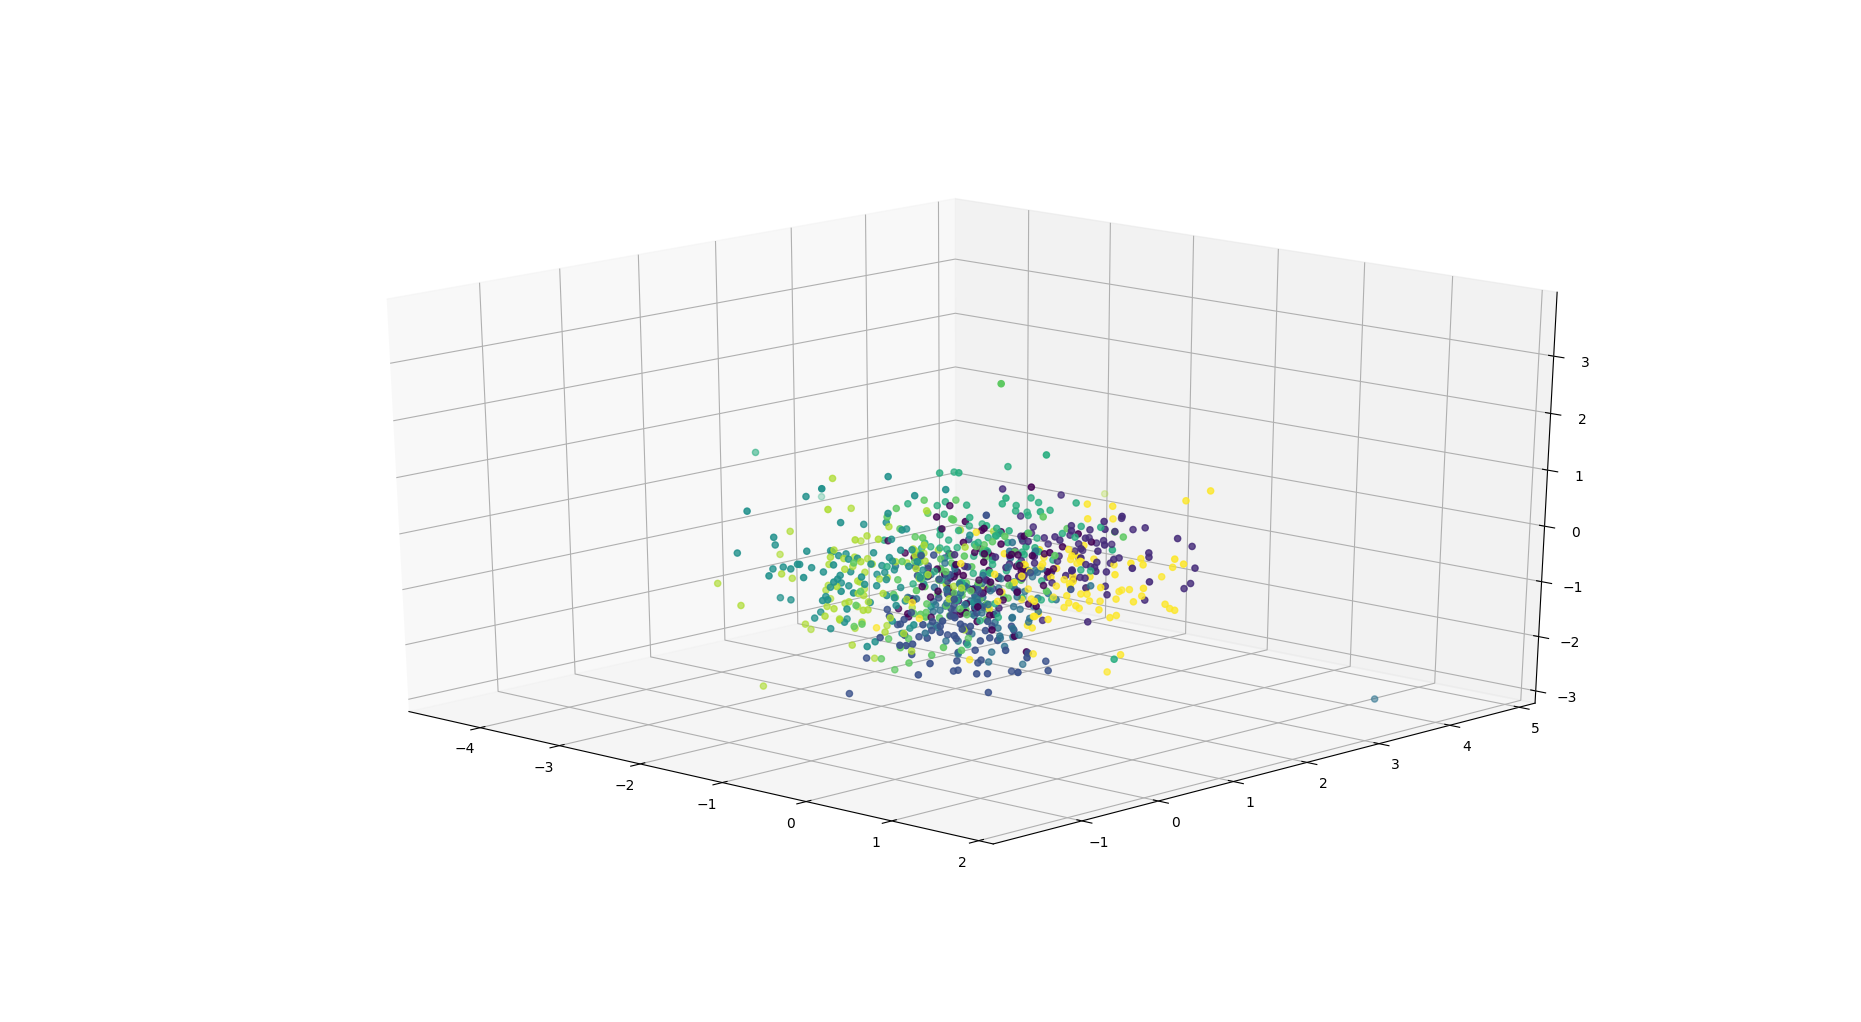
\includegraphics[width=1\linewidth, scale=1]{../img/ej1/oja_corrida_200_9/oja_9salida_200ep_testing_dim123.png}
  \caption{Oja - 9 dimensiones - 200 épocas - Coordenadas 123}
  \label{fig:sub1}
\end{subfigure}%
\begin{subfigure}{.5\textwidth}
  \centering
  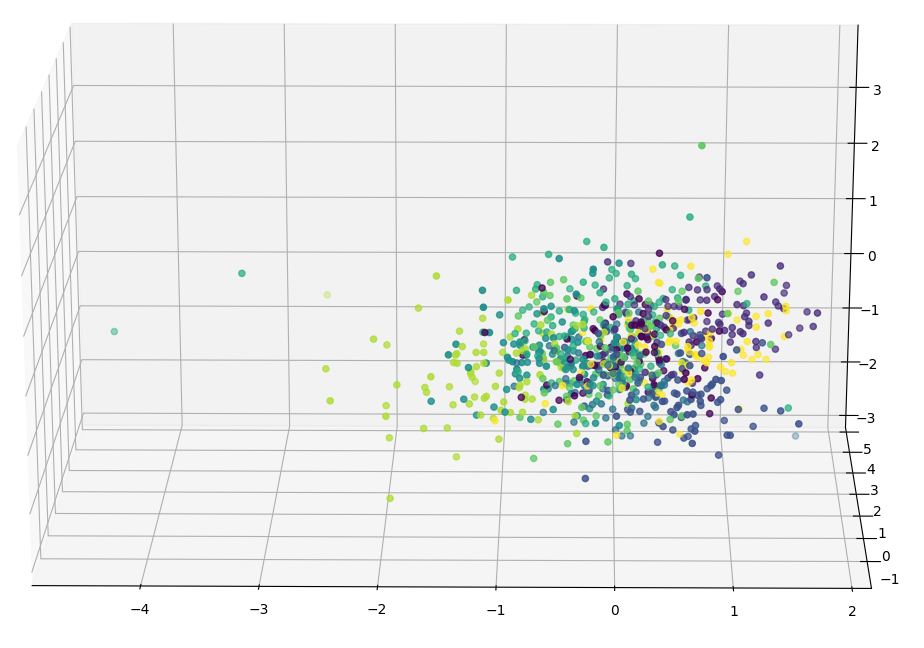
\includegraphics[width=1\linewidth, scale=1]{../img/ej1/oja_corrida_200_9/oja_9salida_200ep_testing_dim123_2.png}
  \caption{Oja - 9 dimensiones - 200 épocas - Coordenadas 123}
  \label{fig:sub2}
\end{subfigure}
\end{figure}

\begin{figure}[!htbp]
\centering
\begin{subfigure}{.5\textwidth}
  \centering
  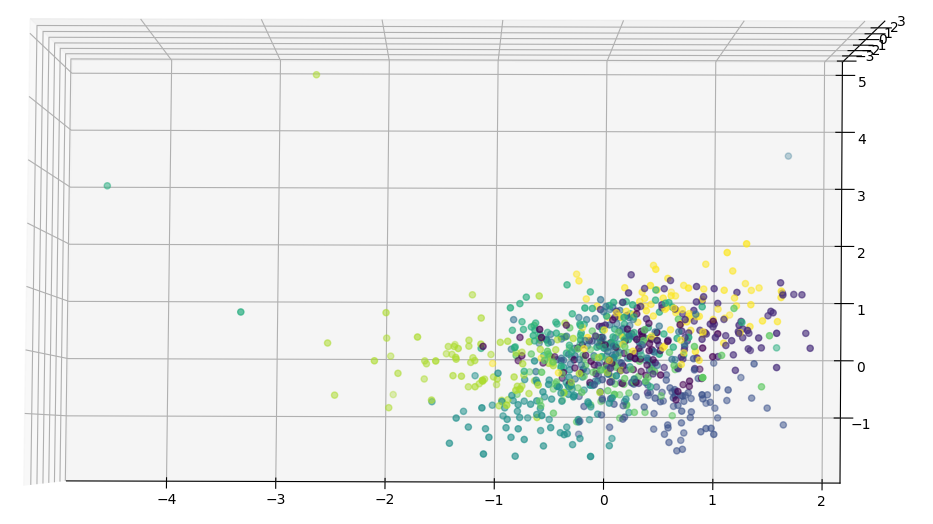
\includegraphics[width=1\linewidth, scale=1]{../img/ej1/oja_corrida_200_9/oja_9salida_200ep_testing_dim123_3.png}
  \caption{Oja - 9 dimensiones - 200 épocas - Coordenadas 123}
  \label{fig:sub1}
\end{subfigure}%
\begin{subfigure}{.5\textwidth}
  \centering
  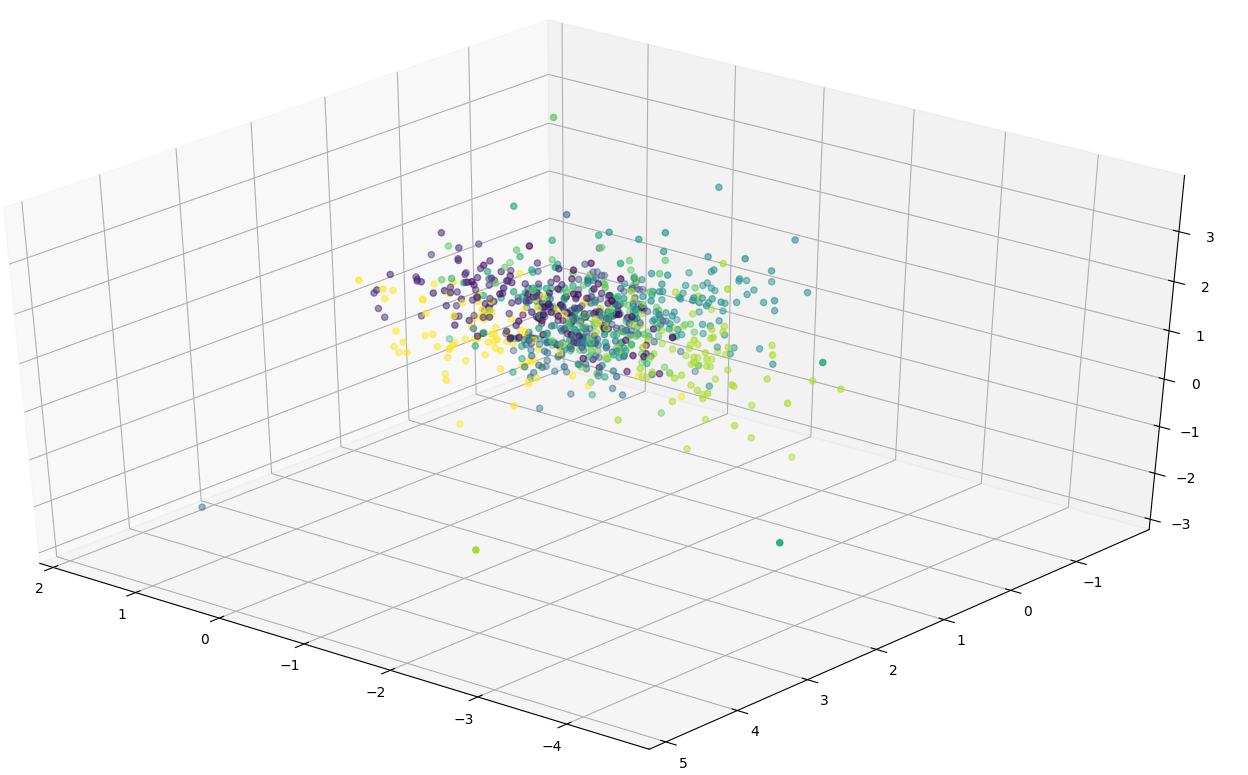
\includegraphics[width=1\linewidth, scale=1]{../img/ej1/oja_corrida_200_9/oja_9salida_200ep_testing_dim123_4.png}
  \caption{Oja - 9 dimensiones - 200 épocas - Coordenadas 123}
  \label{fig:sub2}
\end{subfigure}
\end{figure}

\newpage

En estas primeras 3 coordenadas, los clusters se encuentran muy entrelazados y mezclados, la clasificación no es clara. No se observan demasiadas mejoras
contra la versión de 3 dimensiones únicas.

Veamos las siguientes 3 coordenadas.

\begin{figure}[!htbp]
\centering
\begin{subfigure}{.5\textwidth}
  \centering
  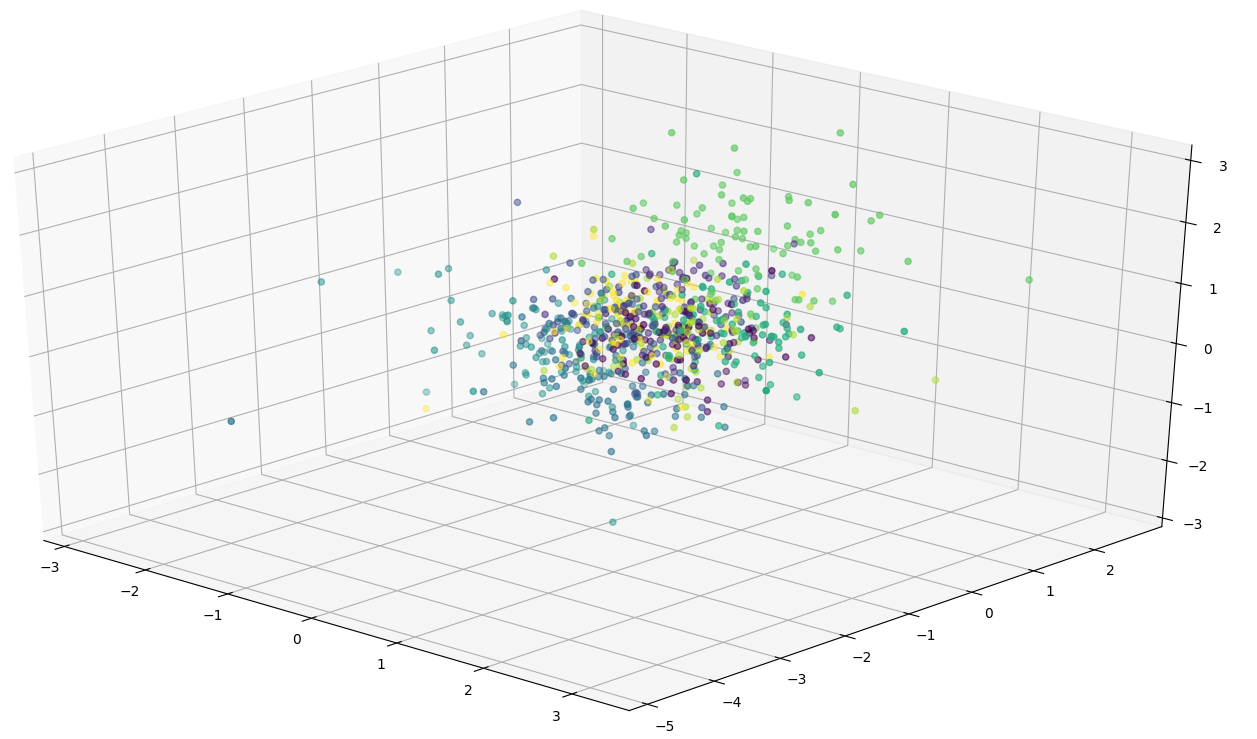
\includegraphics[width=1\linewidth, scale=1]{../img/ej1/oja_corrida_200_9/oja_9salida_200ep_testing_dim456.png}
  \caption{Oja - 9 dimensiones - 200 épocas - Coordenadas 456}
  \label{fig:sub1}
\end{subfigure}%
\begin{subfigure}{.5\textwidth}
  \centering
  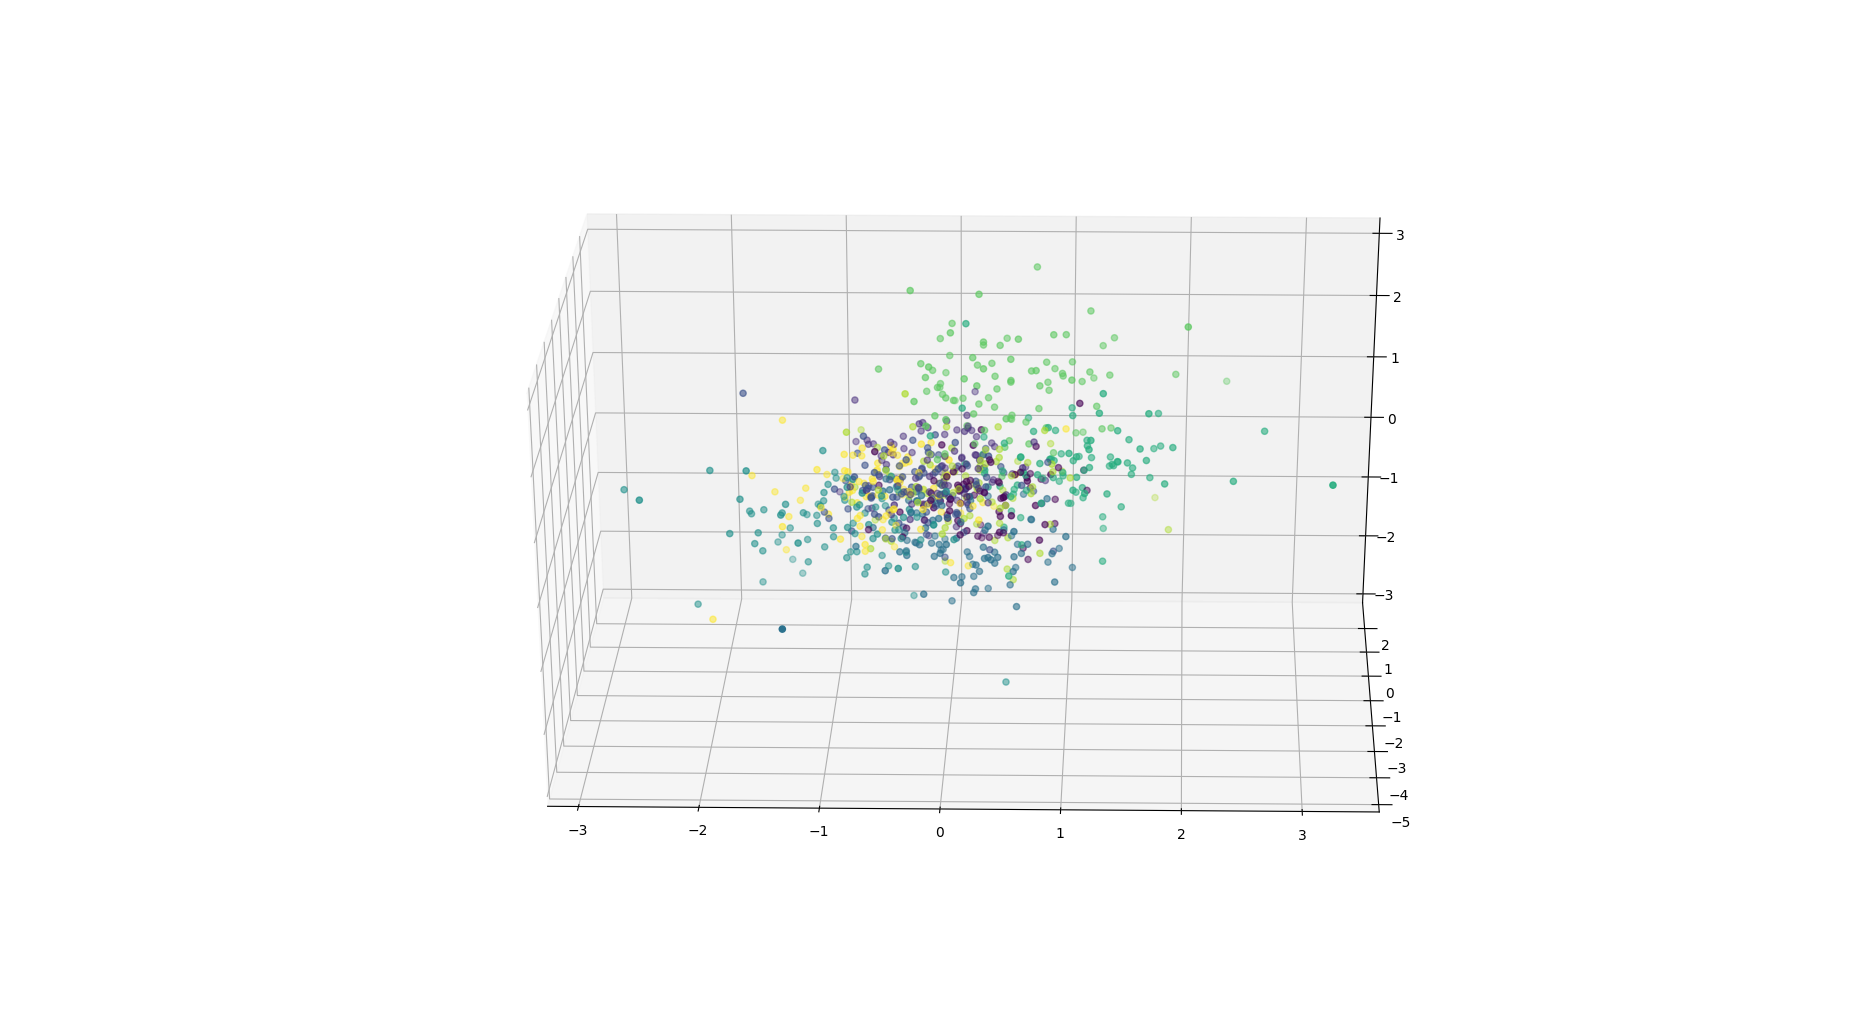
\includegraphics[width=1\linewidth, scale=1]{../img/ej1/oja_corrida_200_9/oja_9salida_200ep_testing_dim456_2.png}
  \caption{Oja - 9 dimensiones - 200 épocas - Coordenadas 456}
  \label{fig:sub2}
\end{subfigure}
\end{figure}

\begin{figure}[!htbp]
\centering
\begin{subfigure}{.5\textwidth}
  \centering
  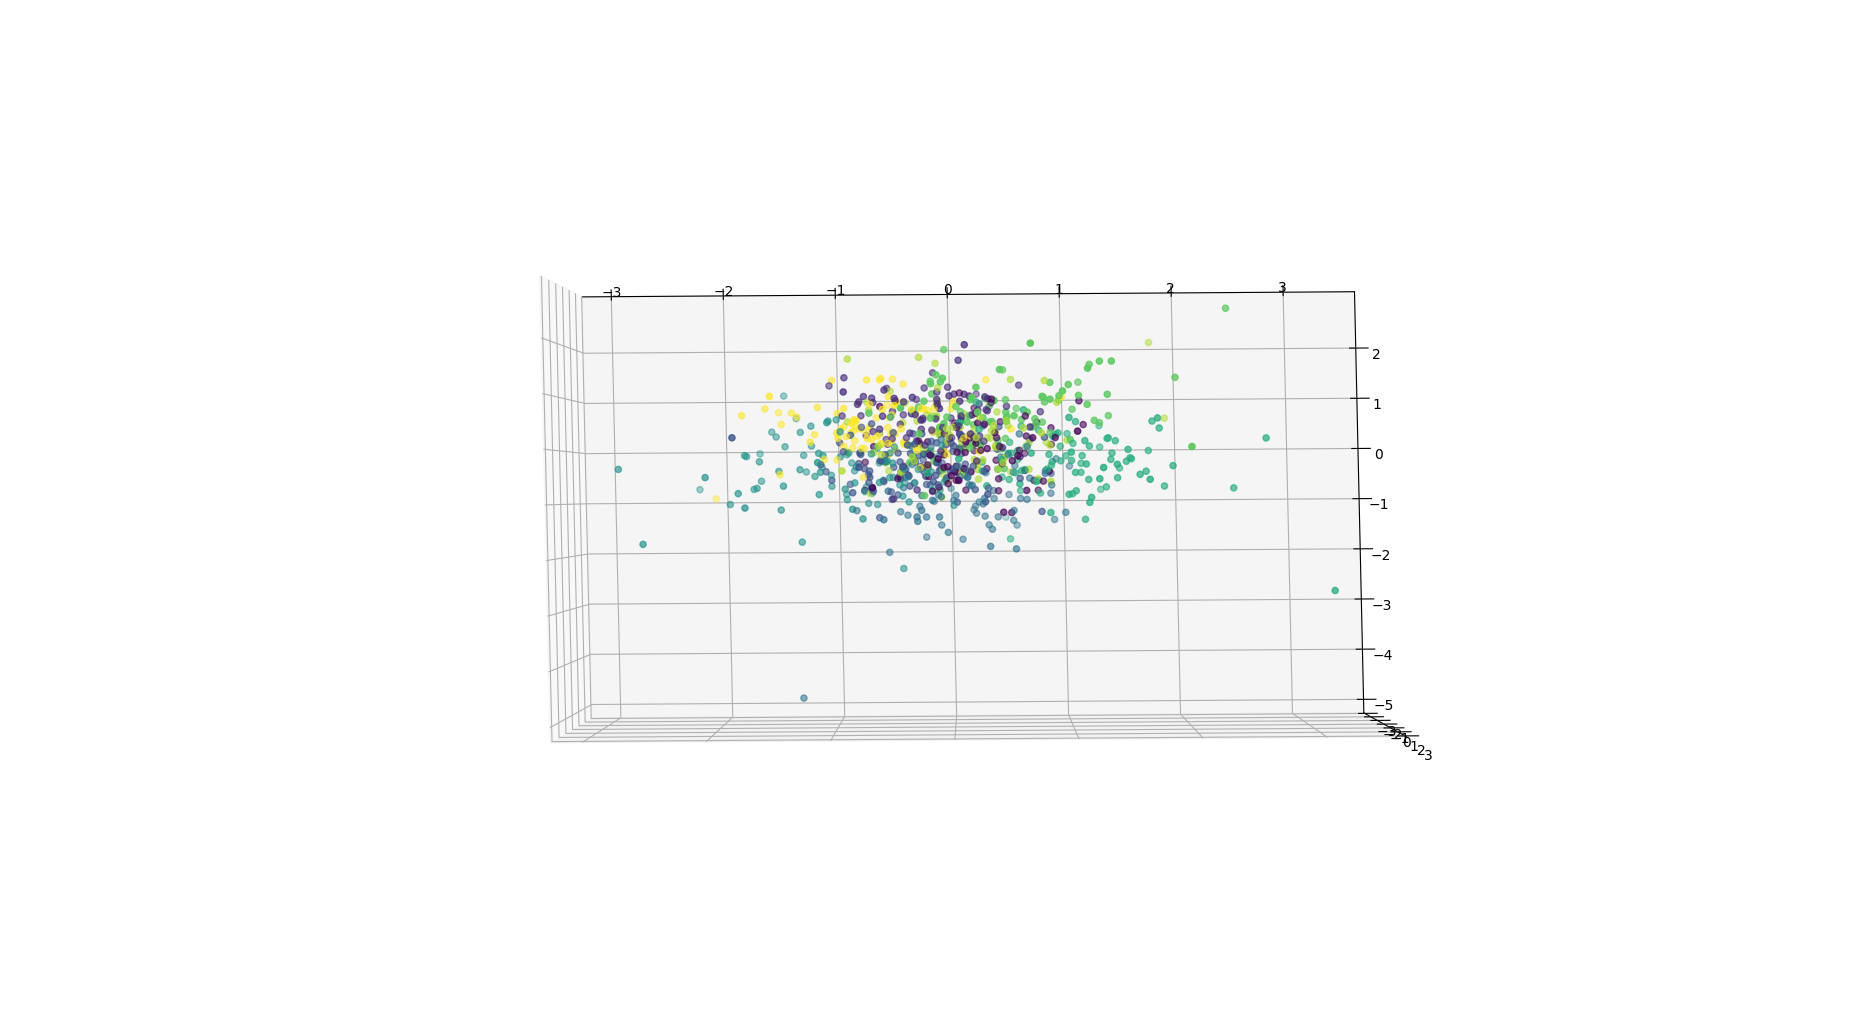
\includegraphics[width=1\linewidth, scale=1]{../img/ej1/oja_corrida_200_9/oja_9salida_200ep_testing_dim456_3.png}
  \caption{Oja - 9 dimensiones - 200 épocas - Coordenadas 456}
  \label{fig:sub1}
\end{subfigure}%
\begin{subfigure}{.5\textwidth}
  \centering
  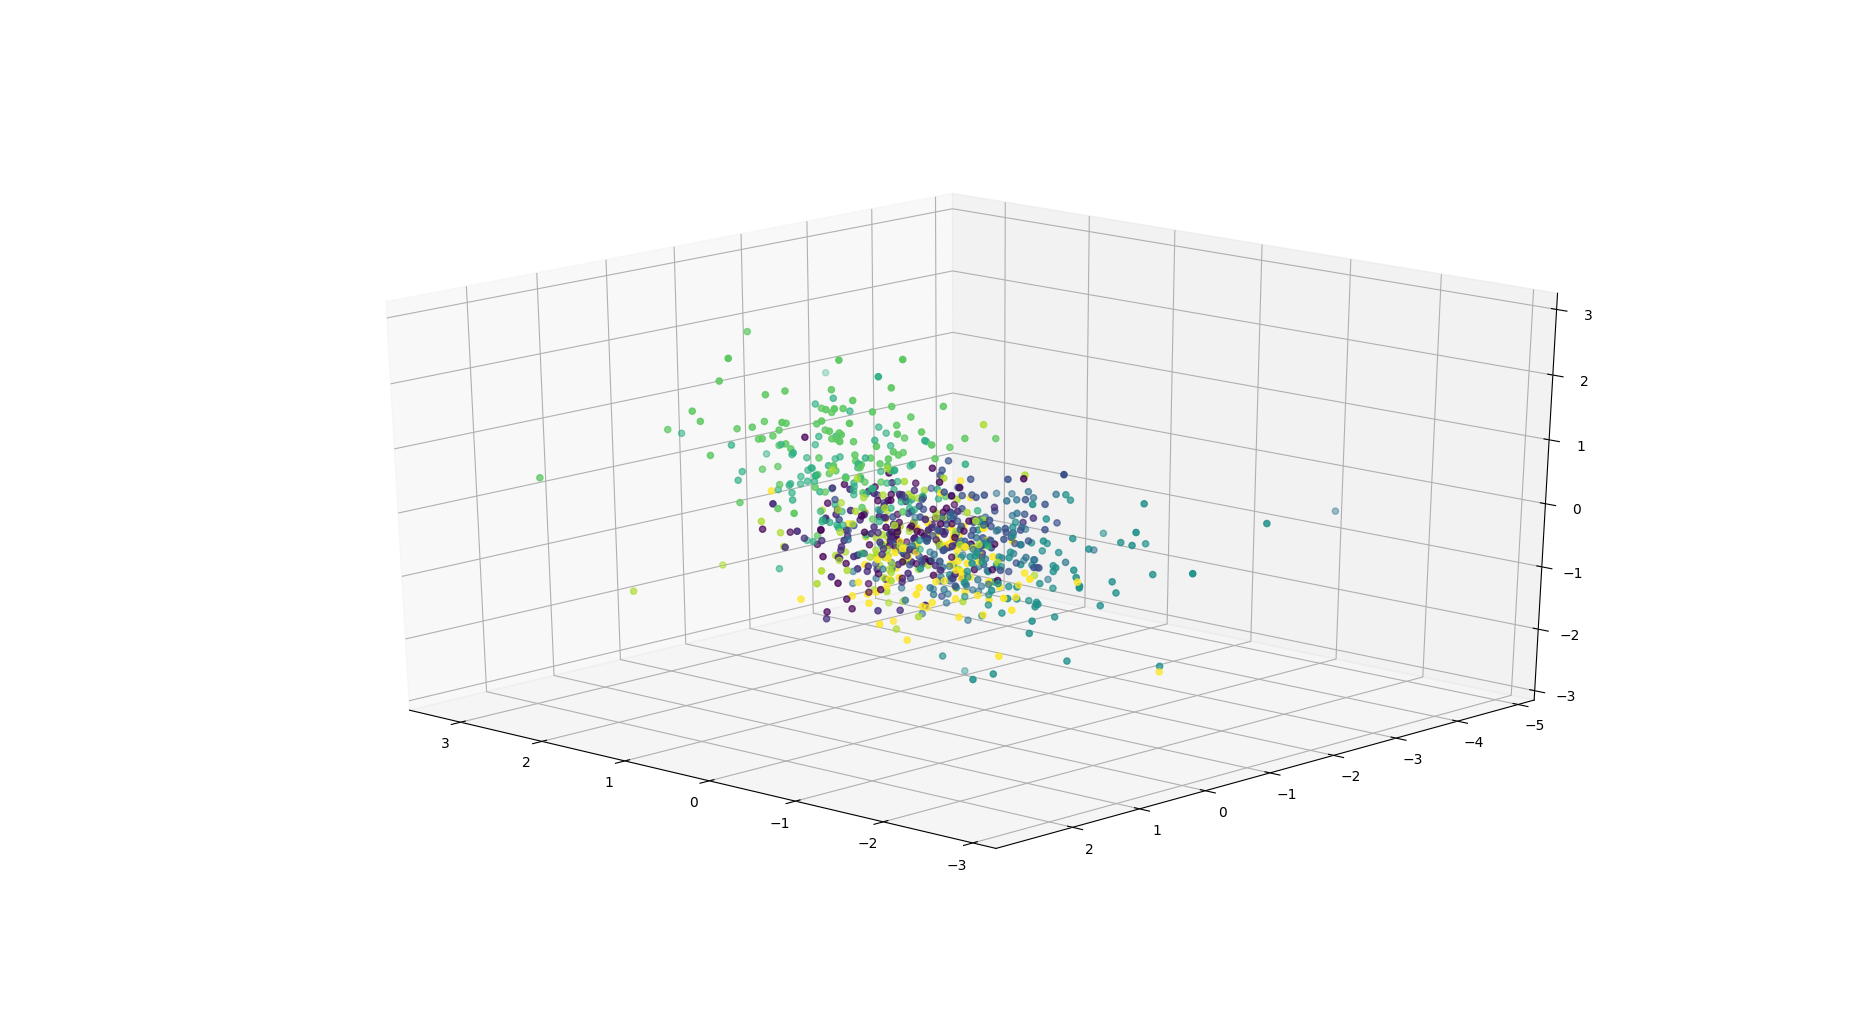
\includegraphics[width=1\linewidth, scale=1]{../img/ej1/oja_corrida_200_9/oja_9salida_200ep_testing_dim456_4.png}
  \caption{Oja - 9 dimensiones - 200 épocas - Coordenadas 456}
  \label{fig:sub2}
\end{subfigure}
\end{figure}

Para las coordenadas 456 vemos que hay una mayor expansión del espacio ocupado por los datos y se nota un grado levemente mayor de separación entre
los puntos coloreados.

Veamos las siguientes 3 coordenadas.

\begin{figure}[!htbp]
\centering
\begin{subfigure}{.5\textwidth}
  \centering
  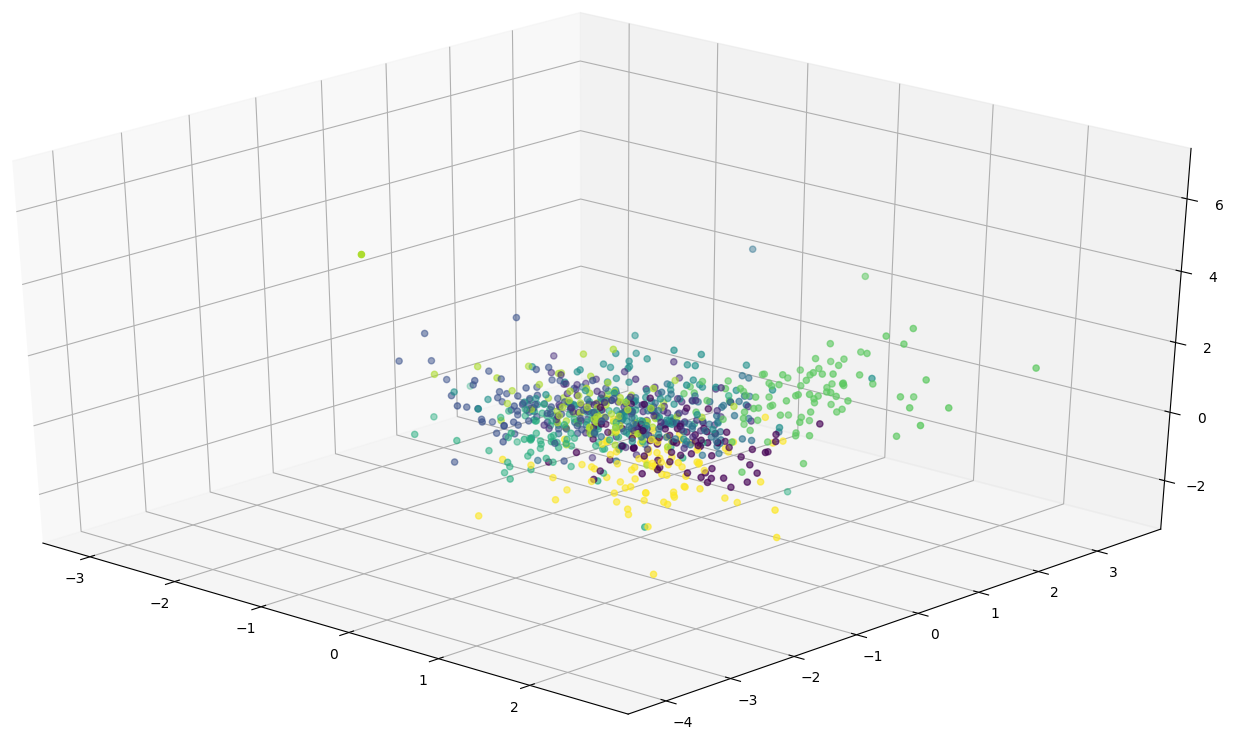
\includegraphics[width=1\linewidth, scale=1]{../img/ej1/oja_corrida_200_9/oja_9salida_200ep_testing_dim789.png}
  \caption{Oja - 9 dimensiones - 200 épocas - Coordenadas 789}
  \label{fig:sub1}
\end{subfigure}%
\begin{subfigure}{.5\textwidth}
  \centering
  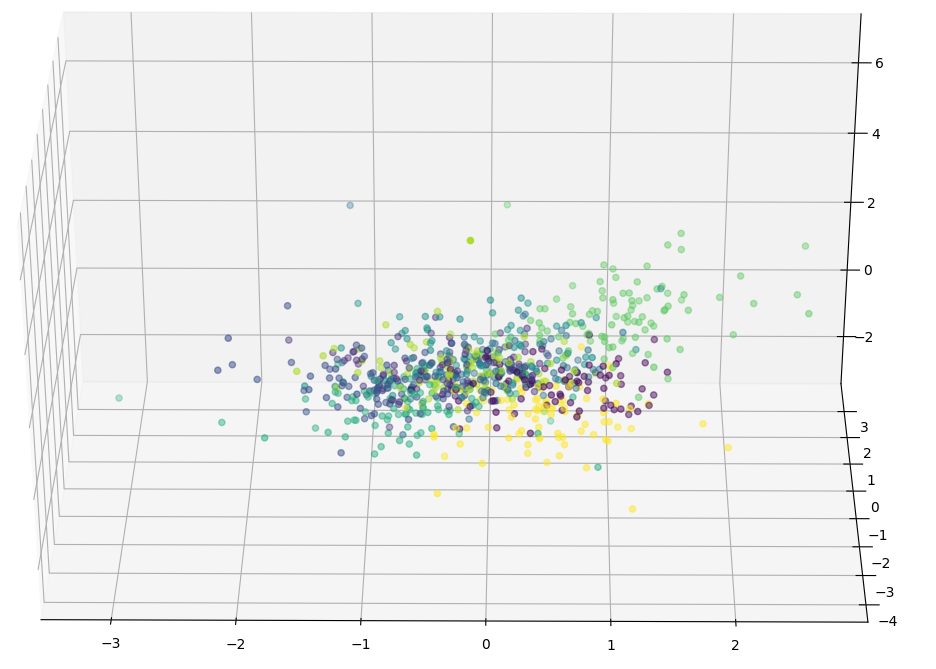
\includegraphics[width=1\linewidth, scale=1]{../img/ej1/oja_corrida_200_9/oja_9salida_200ep_testing_dim789_2.png}
  \caption{Oja - 9 dimensiones - 200 épocas - Coordenadas 789}
  \label{fig:sub2}
\end{subfigure}
\end{figure}

\begin{figure}[!htbp]
\centering
\begin{subfigure}{.5\textwidth}
  \centering
  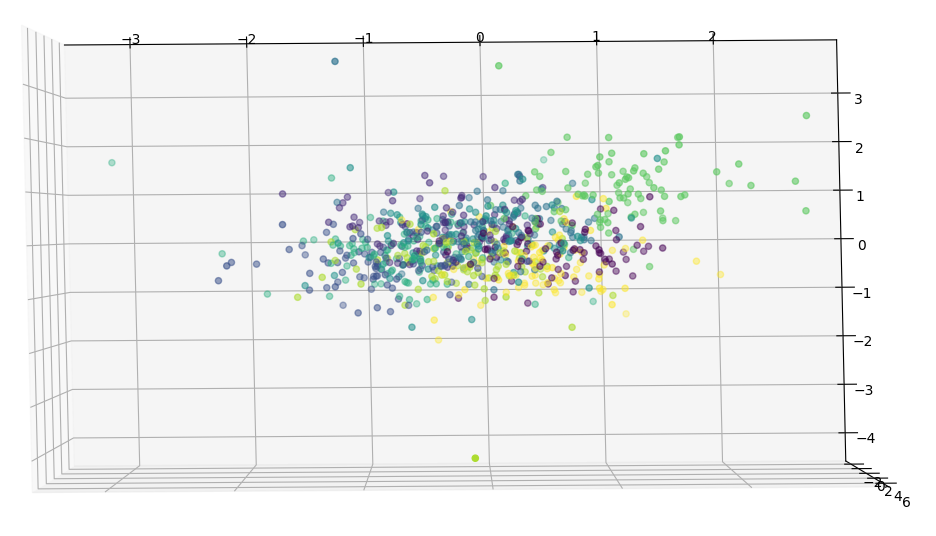
\includegraphics[width=1\linewidth, scale=1]{../img/ej1/oja_corrida_200_9/oja_9salida_200ep_testing_dim789_3.png}
  \caption{Oja - 9 dimensiones - 200 épocas - Coordenadas 789}
  \label{fig:sub1}
\end{subfigure}%
\begin{subfigure}{.5\textwidth}
  \centering
  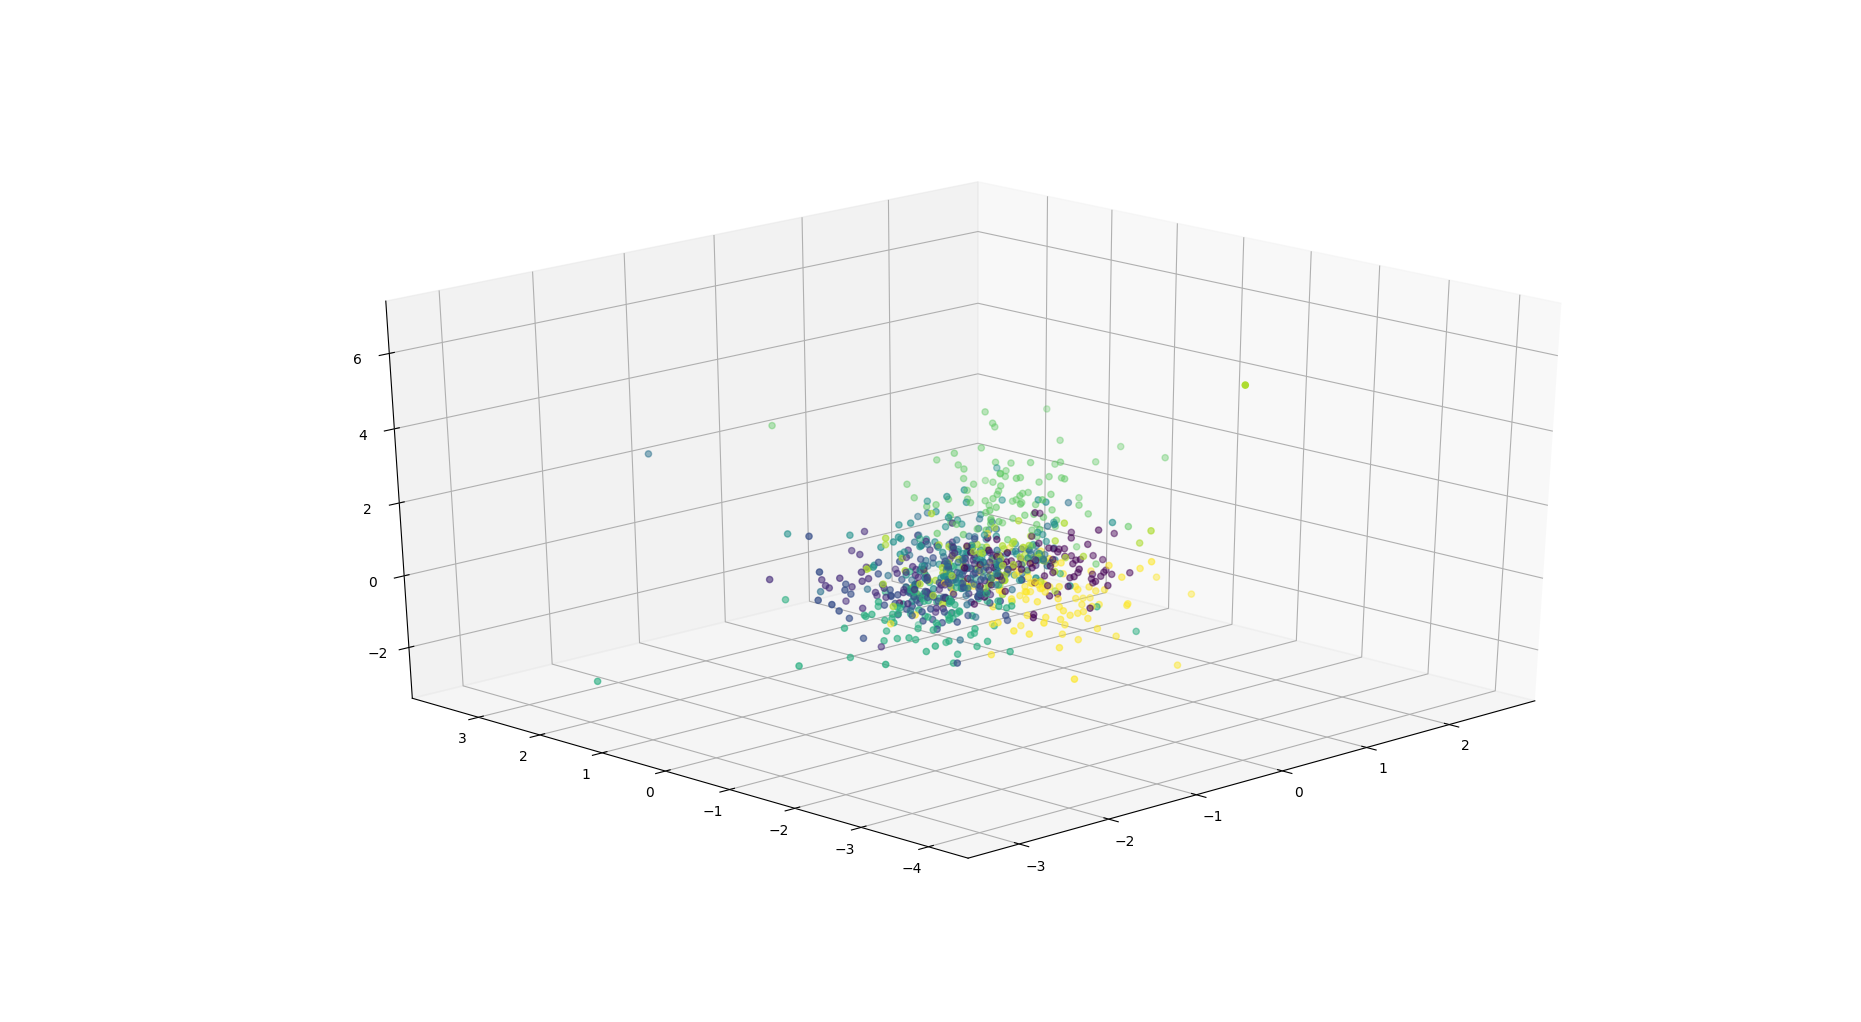
\includegraphics[width=1\linewidth, scale=1]{../img/ej1/oja_corrida_200_9/oja_9salida_200ep_testing_dim789_4.png}
  \caption{Oja - 9 dimensiones - 200 épocas - Coordenadas 789}
  \label{fig:sub2}
\end{subfigure}
\end{figure}

En las últimas coordenadas los resultados son similares a las 456. Se notan algunas zonas donde predominan cierta categoría, con bastante solapamiento en la zona central.
Los resultados no se muestran muy superiores a los obtenidos con solo 3 coordenadas totales.

Observemos las ejecuciones utilizando Regla de Sanger.

\subsubsection{Regla de Sanger - Variando número de dimensiones}

\begin{figure}[!htbp]
\centering
\begin{subfigure}{.5\textwidth}
  \centering
  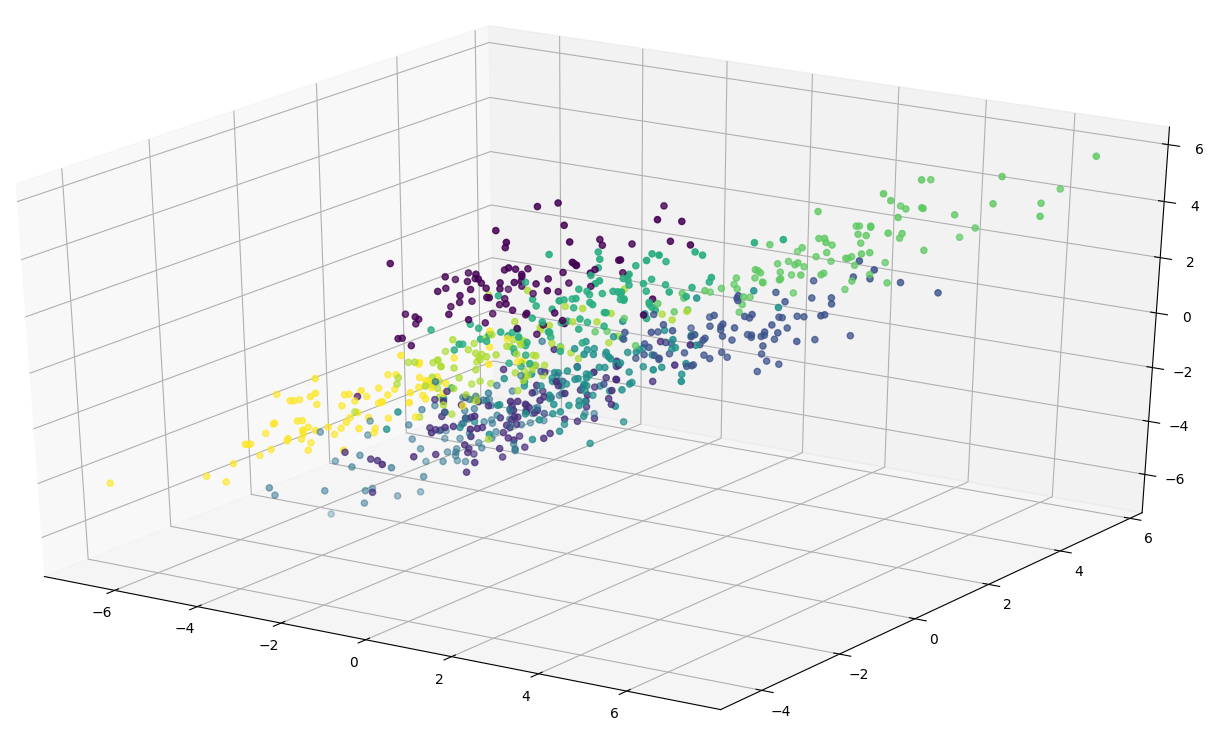
\includegraphics[width=1\linewidth, scale=1]{../img/ej1/sanger_corrida_200_9/sanger_9salida_200ep_testing_dim123.png}
  \caption{Sanger - 9 dimensiones - 200 épocas - Coordenadas 123}
  \label{fig:sub1}
\end{subfigure}%
\begin{subfigure}{.5\textwidth}
  \centering
  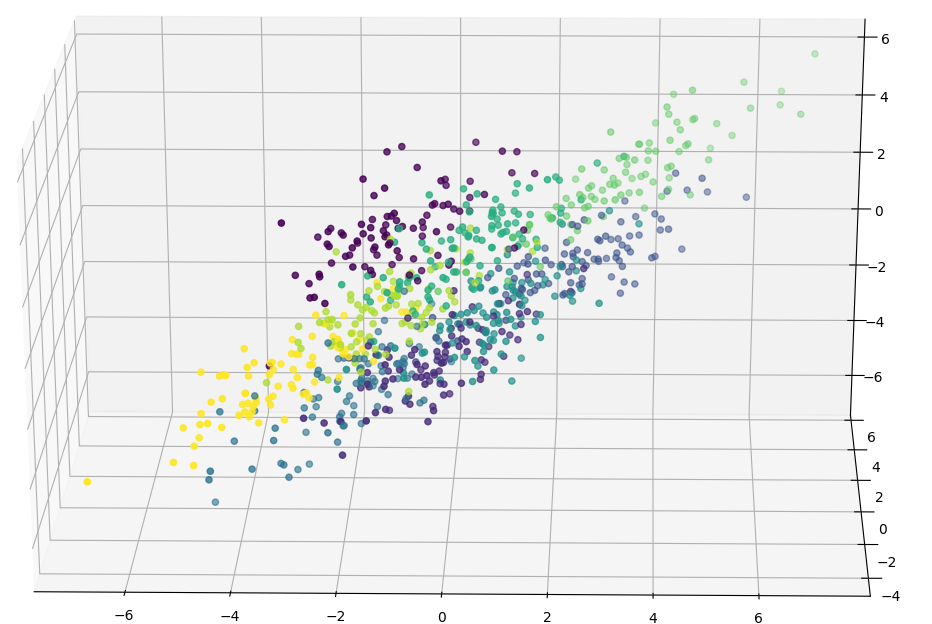
\includegraphics[width=1\linewidth, scale=1]{../img/ej1/sanger_corrida_200_9/sanger_9salida_200ep_testing_dim123_2.png}
  \caption{Sanger - 9 dimensiones - 200 épocas - Coordenadas 123}
  \label{fig:sub2}
\end{subfigure}
\end{figure}

\begin{figure}[!htbp]
\centering
\begin{subfigure}{.5\textwidth}
  \centering
  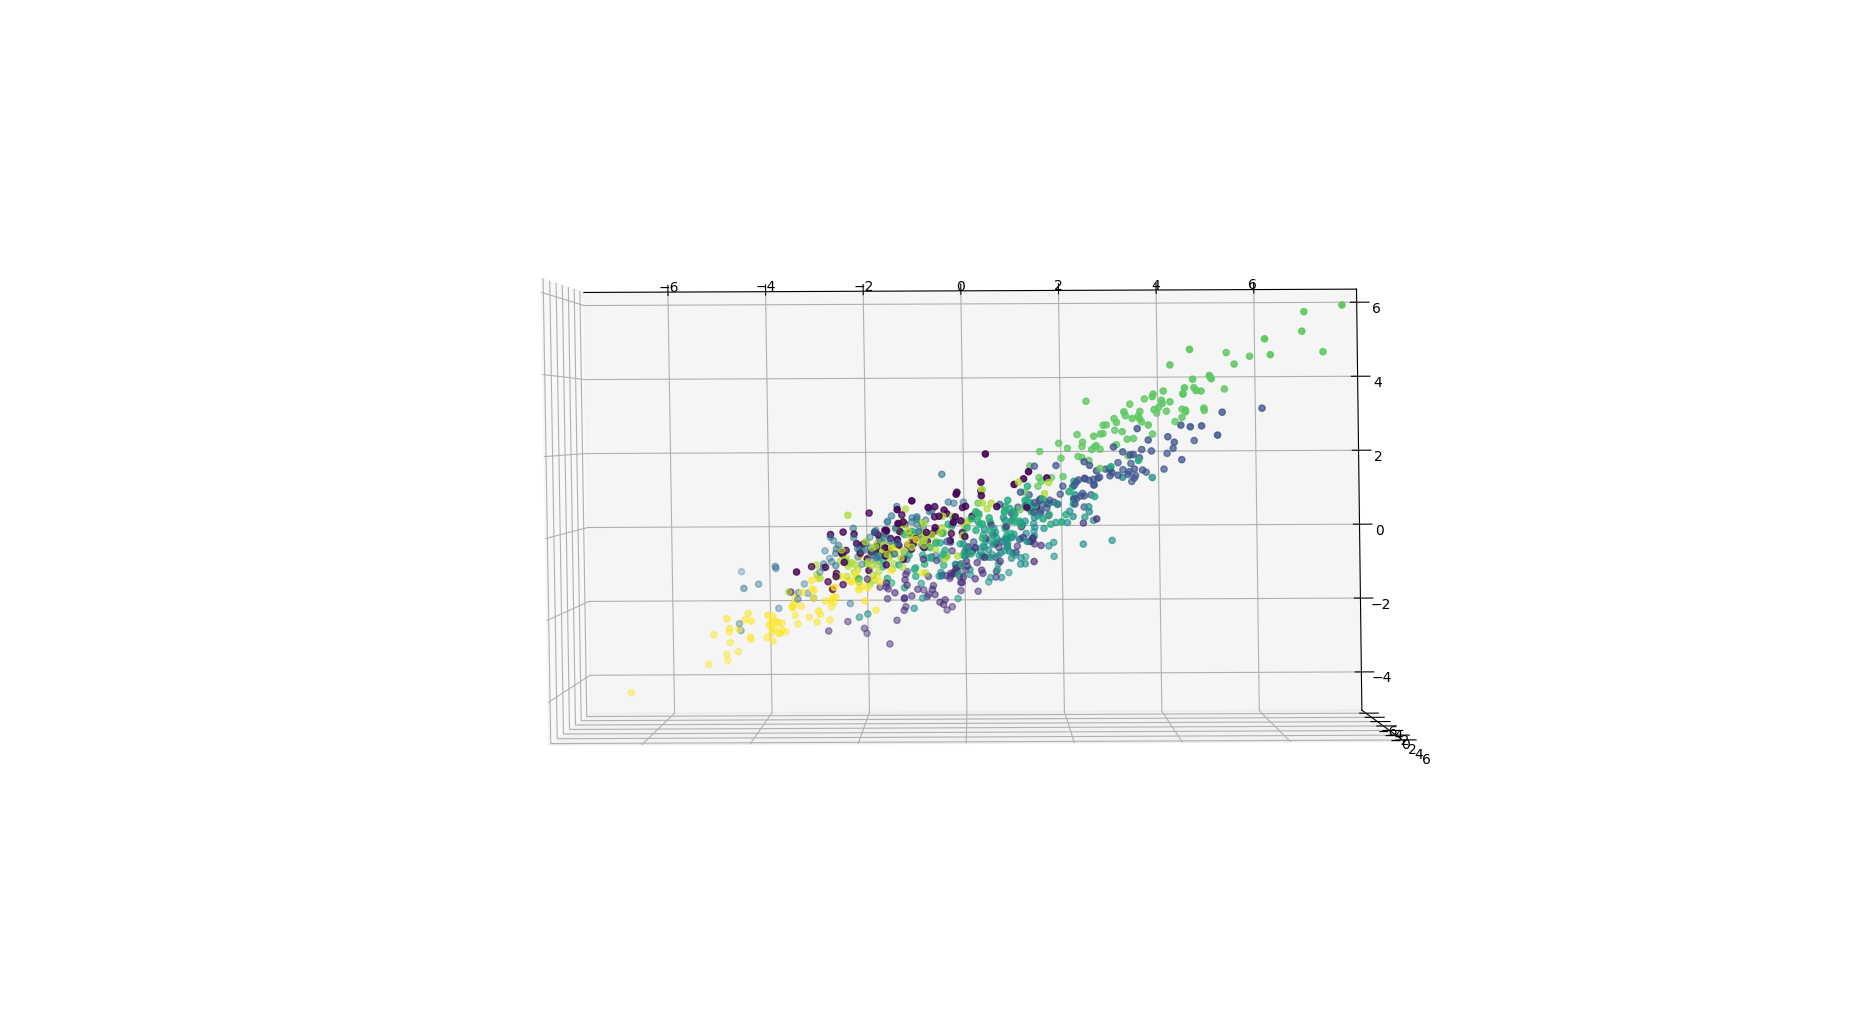
\includegraphics[width=1\linewidth, scale=1]{../img/ej1/sanger_corrida_200_9/sanger_9salida_200ep_testing_dim123_3.png}
  \caption{Sanger - 9 dimensiones - 200 épocas - Coordenadas 123}
  \label{fig:sub1}
\end{subfigure}%
\begin{subfigure}{.5\textwidth}
  \centering
  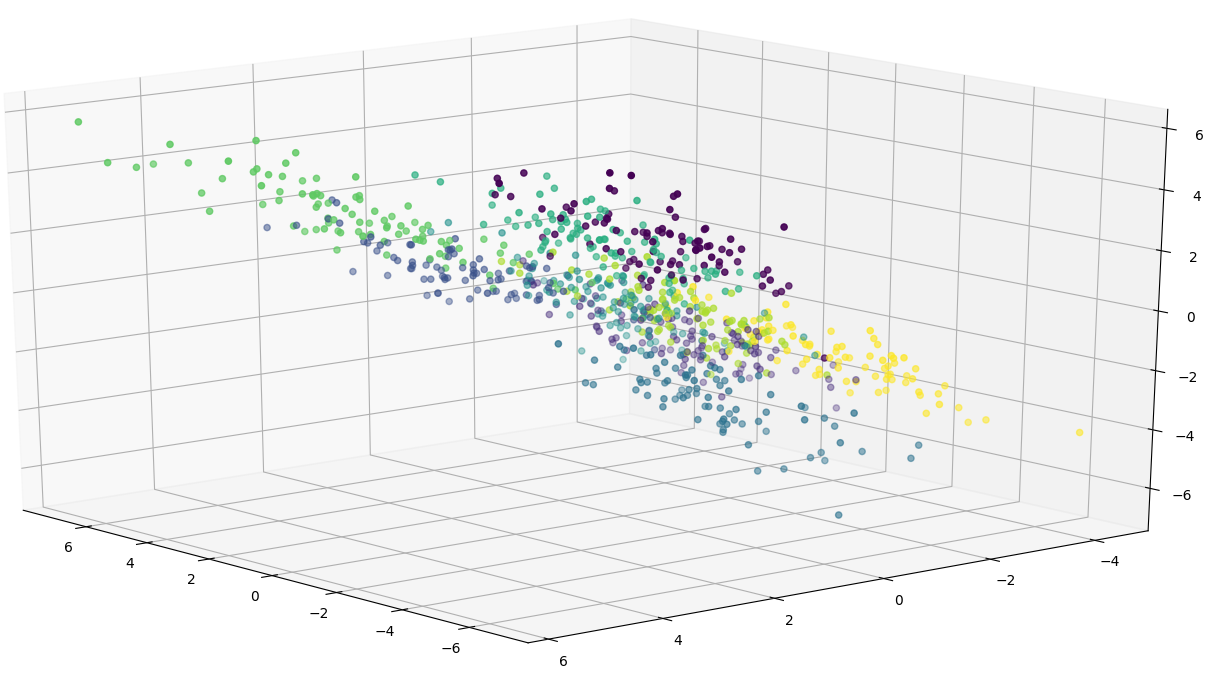
\includegraphics[width=1\linewidth, scale=1]{../img/ej1/sanger_corrida_200_9/sanger_9salida_200ep_testing_dim123_4.png}
  \caption{Sanger - 9 dimensiones - 200 épocas - Coordenadas 123}
  \label{fig:sub2}
\end{subfigure}
\end{figure}

Usando la regla de Sanger se observan mucho mejores resultados. Se pueden observar los clusters separados con mucha mayor claridad. 

A continuación los resultados de las coordenadas 456:

\begin{figure}[!htbp]
\centering
\begin{subfigure}{.5\textwidth}
  \centering
  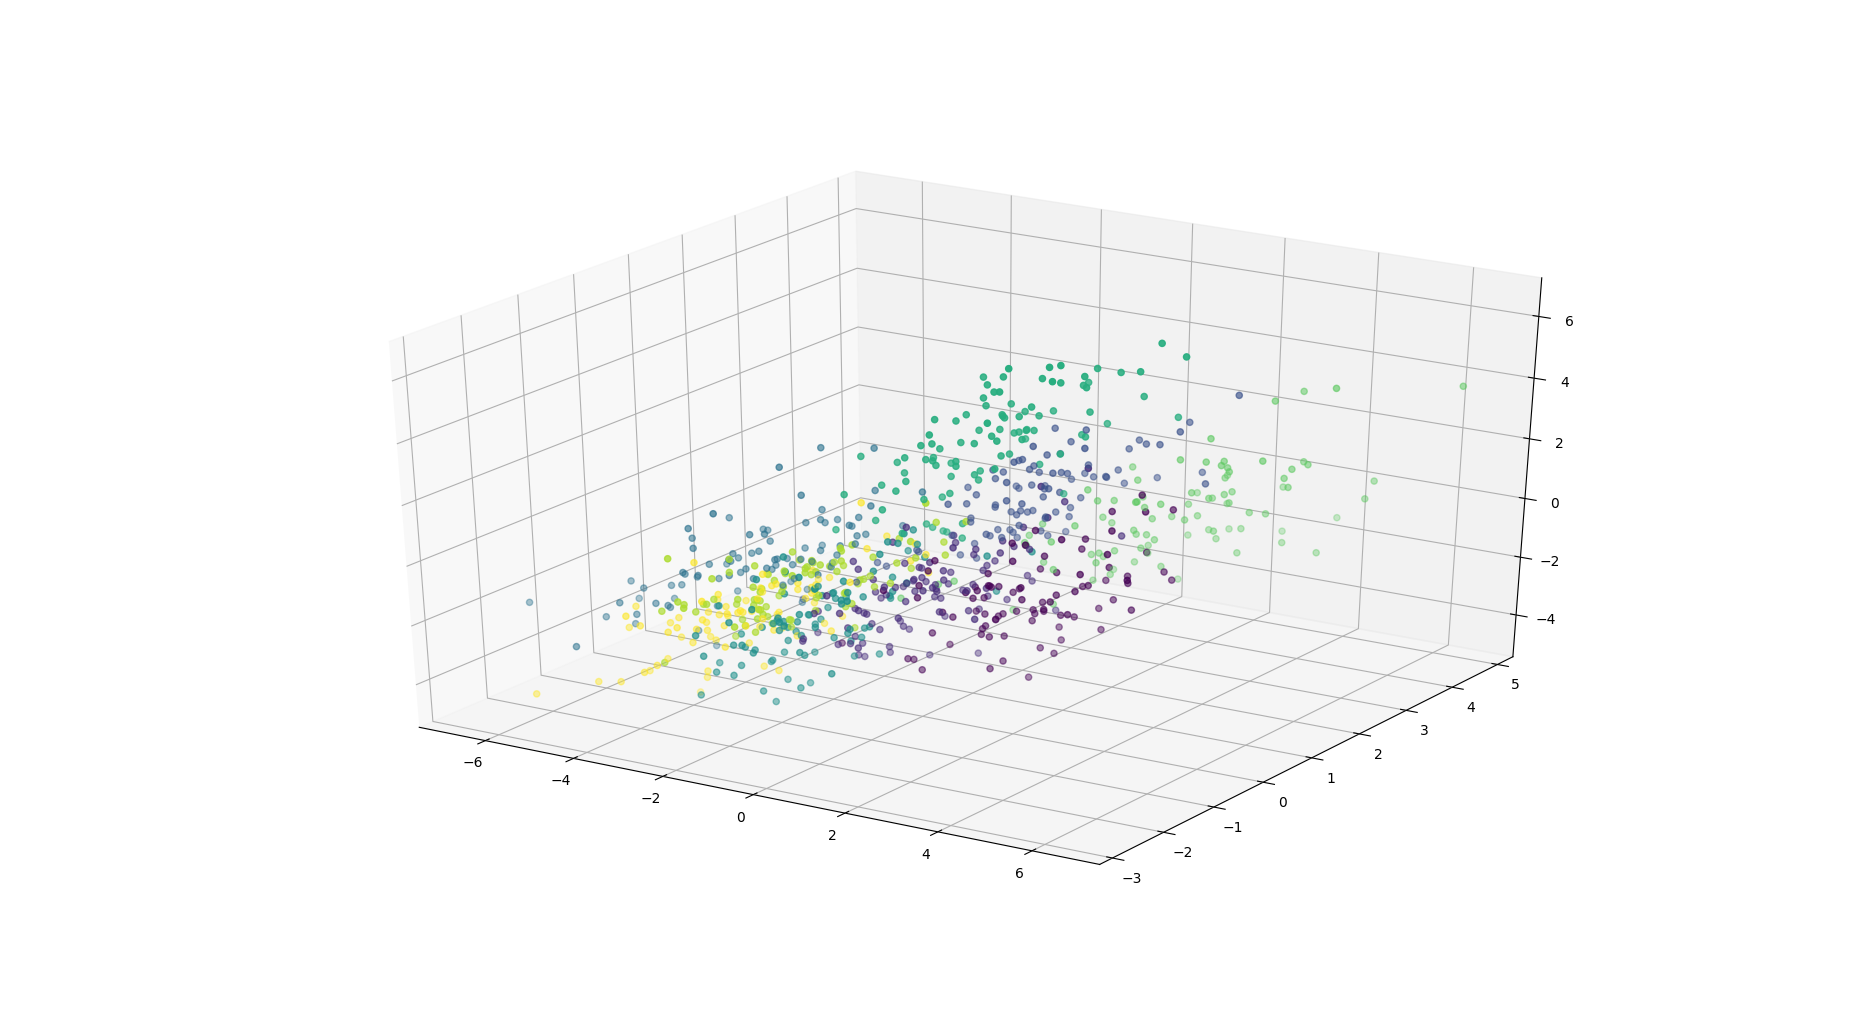
\includegraphics[width=1\linewidth, scale=1]{../img/ej1/sanger_corrida_200_9/sanger_9salida_200ep_testing_dim456.png}
  \caption{Sanger - 9 dimensiones - 200 épocas - Coordenadas 456}
  \label{fig:sub1}
\end{subfigure}%
\begin{subfigure}{.5\textwidth}
  \centering
  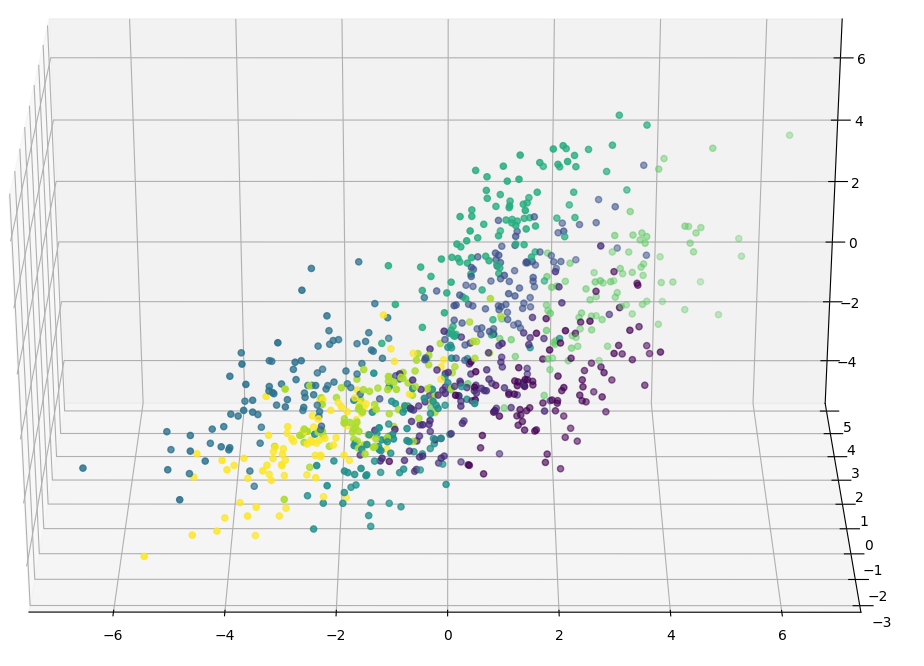
\includegraphics[width=1\linewidth, scale=1]{../img/ej1/sanger_corrida_200_9/sanger_9salida_200ep_testing_dim456_2.png}
  \caption{Sanger - 9 dimensiones - 200 épocas - Coordenadas 456}
  \label{fig:sub2}
\end{subfigure}
\end{figure}

\begin{figure}[!htbp]
\centering
\begin{subfigure}{.5\textwidth}
  \centering
  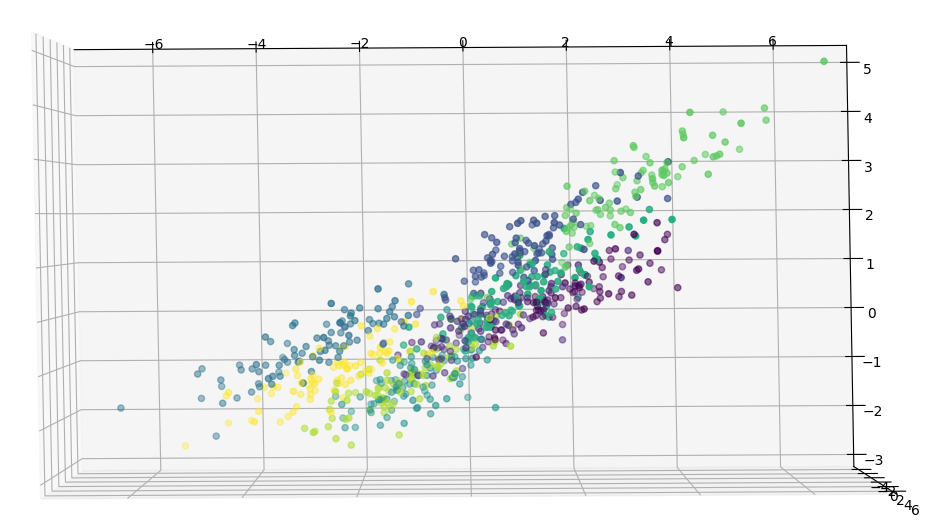
\includegraphics[width=1\linewidth, scale=1]{../img/ej1/sanger_corrida_200_9/sanger_9salida_200ep_testing_dim456_3.png}
  \caption{Sanger - 9 dimensiones - 200 épocas - Coordenadas 456}
  \label{fig:sub1}
\end{subfigure}%
\begin{subfigure}{.5\textwidth}
  \centering
  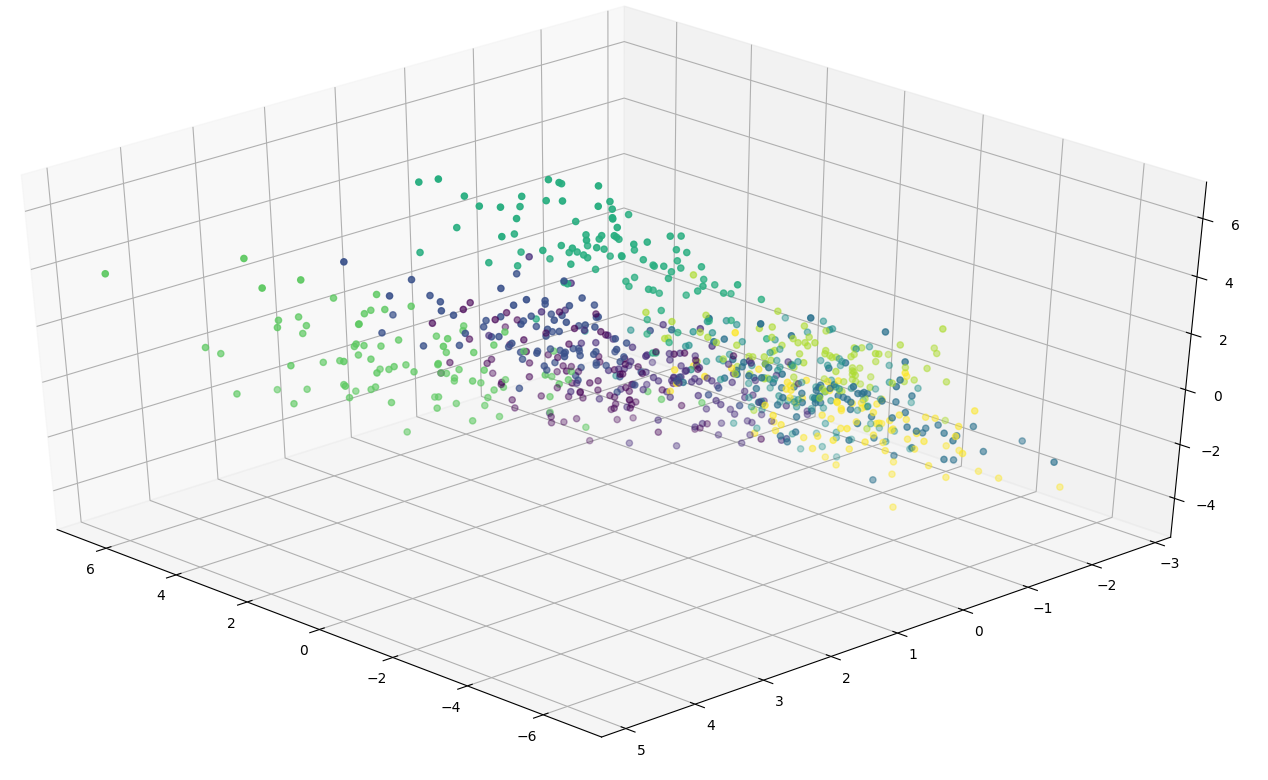
\includegraphics[width=1\linewidth, scale=1]{../img/ej1/sanger_corrida_200_9/sanger_9salida_200ep_testing_dim456_4.png}
  \caption{Sanger - 9 dimensiones - 200 épocas - Coordenadas 456}
  \label{fig:sub2}
\end{subfigure}
\end{figure}

En esta tanda vemos nuevamente una clasificación más marcada y con mayor espacio entre los clusters. Se puede apreciar la agrupación
de las marcas del mismo color, mostrando la asociación entre documentos de la misma categoría.

Veamos las últimas 3 coordenadas.


\begin{figure}[!htbp]
\centering
\begin{subfigure}{.5\textwidth}
  \centering
  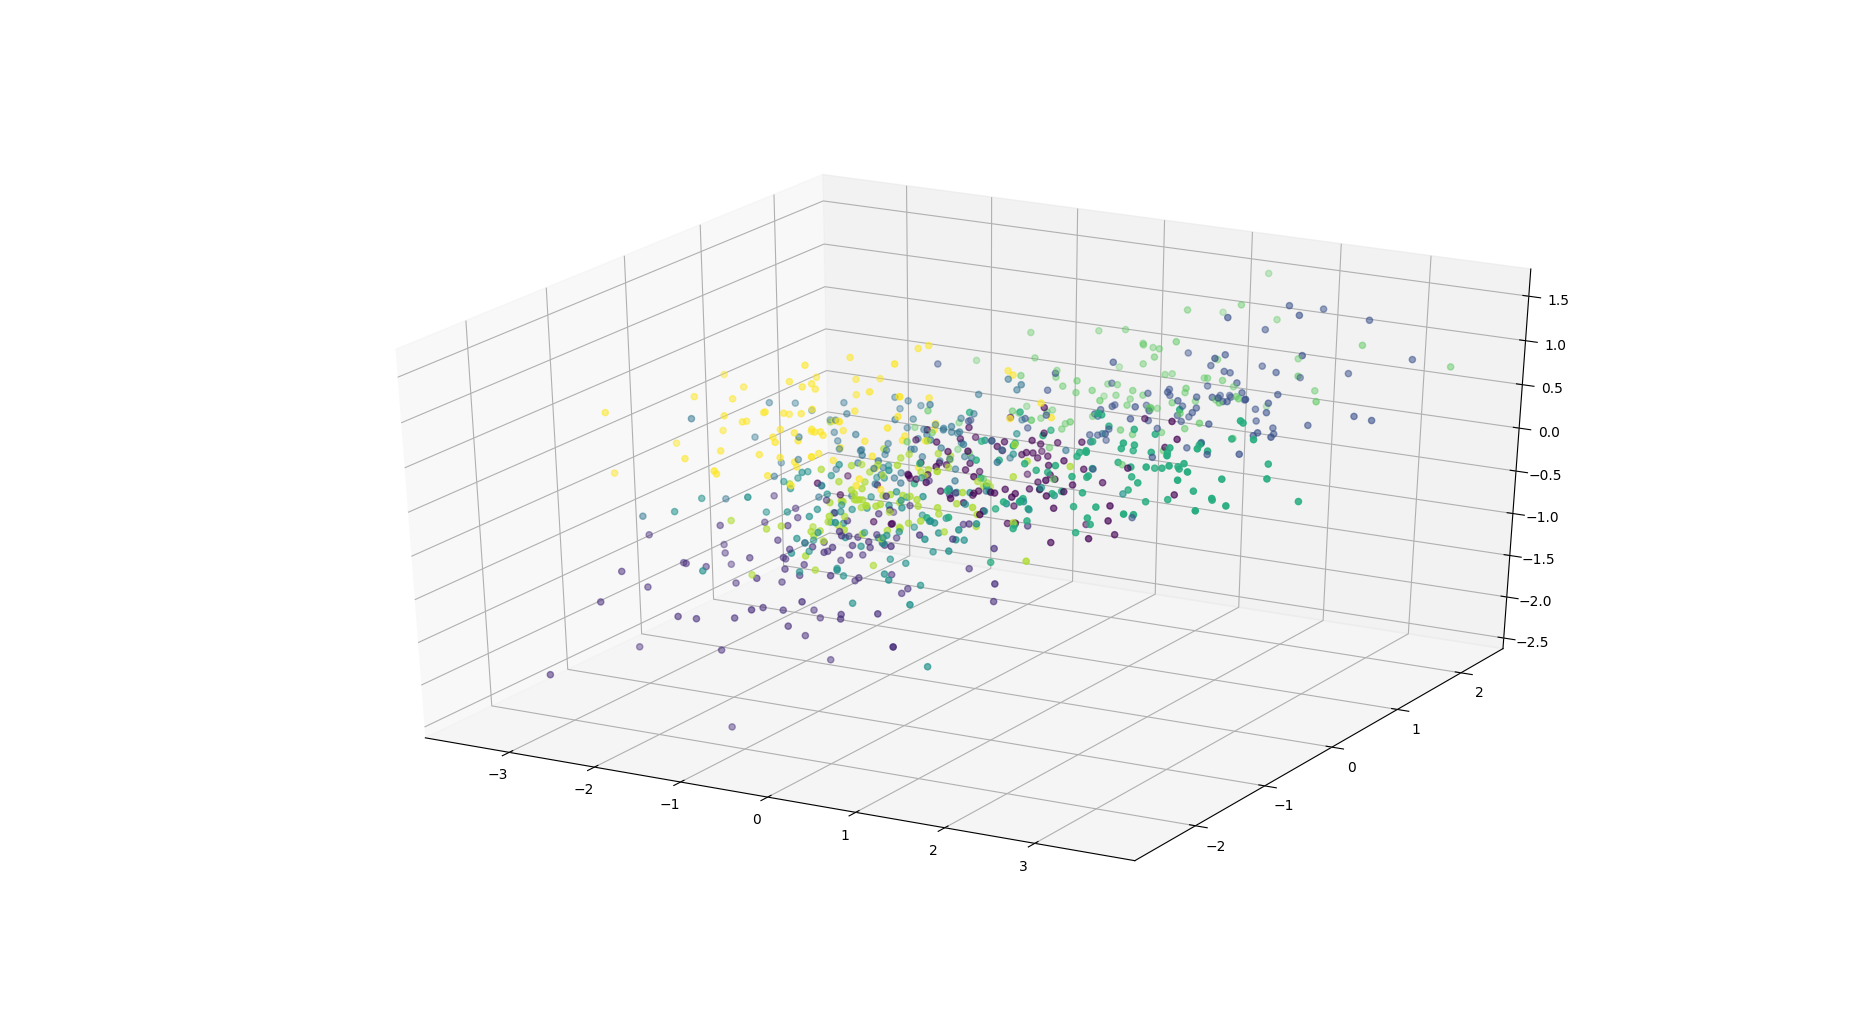
\includegraphics[width=1\linewidth, scale=1]{../img/ej1/sanger_corrida_200_9/sanger_9salida_200ep_testing_dim789.png}
  \caption{Sanger - 9 dimensiones - 200 épocas - Coordenadas 789}
  \label{fig:sub1}
\end{subfigure}%
\begin{subfigure}{.5\textwidth}
  \centering
  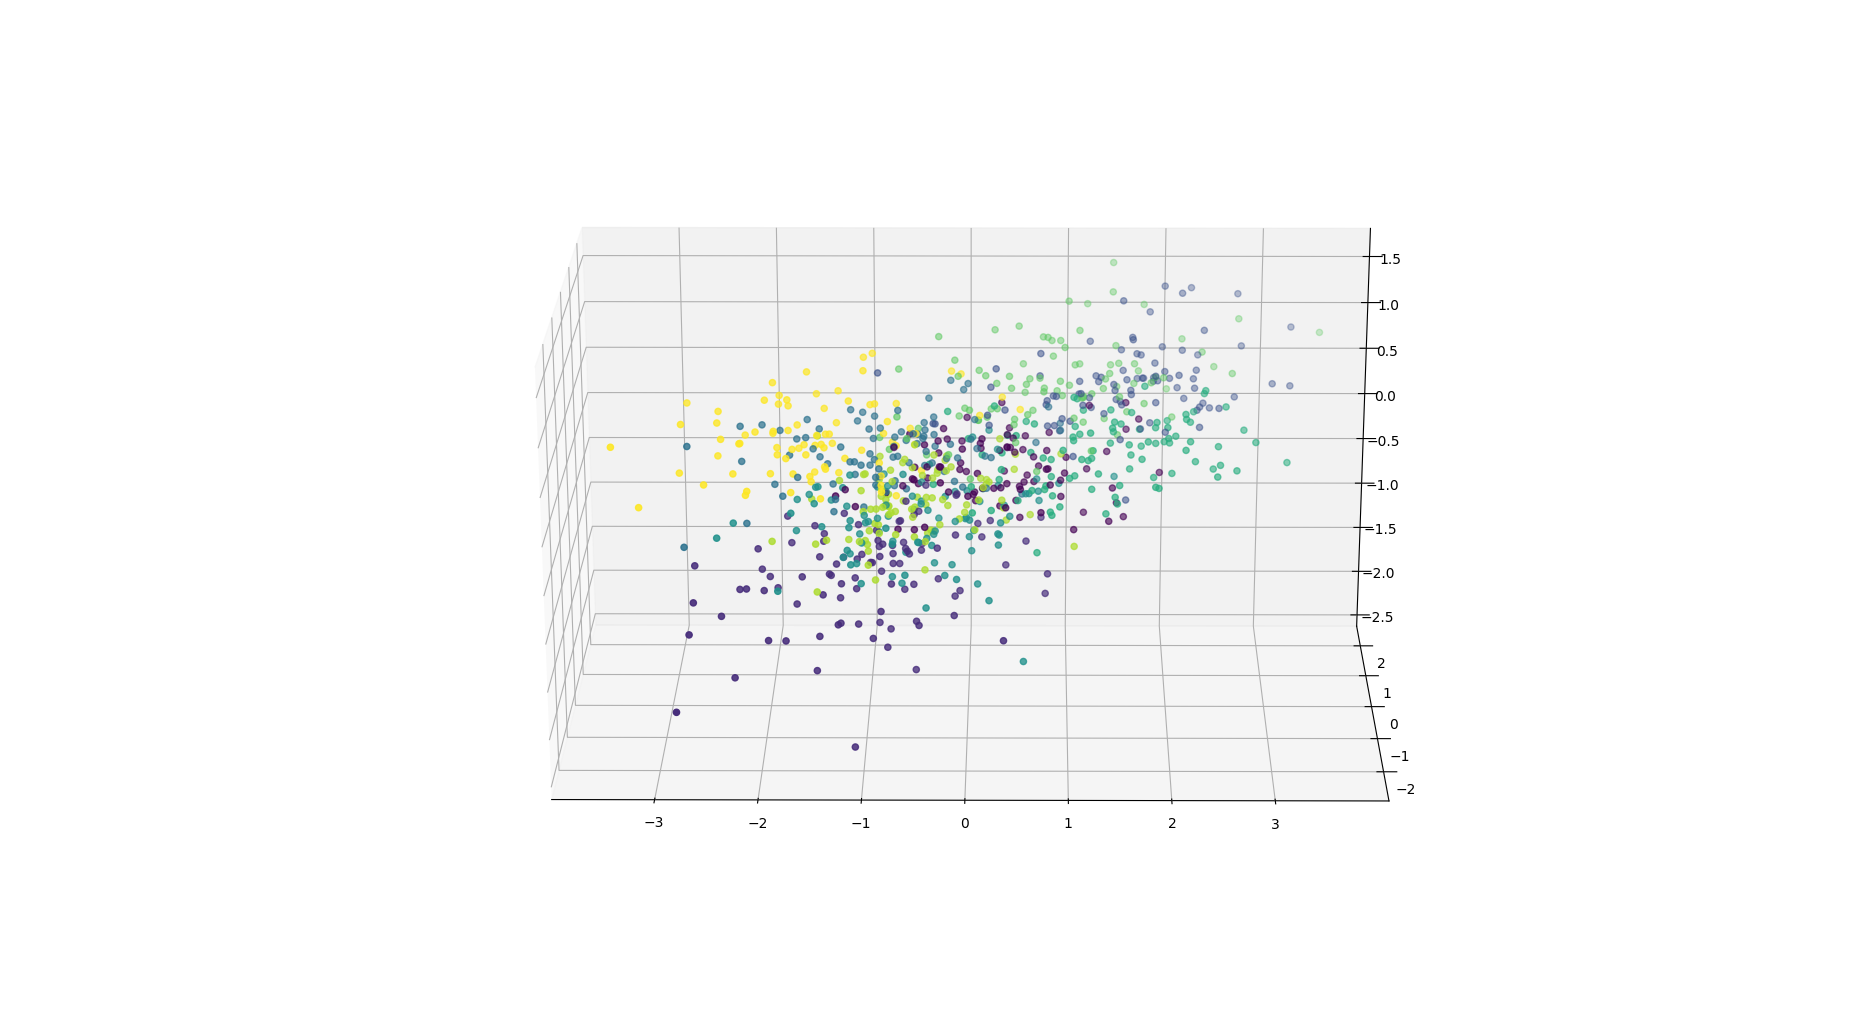
\includegraphics[width=1\linewidth, scale=1]{../img/ej1/sanger_corrida_200_9/sanger_9salida_200ep_testing_dim789_2.png}
  \caption{Sanger - 9 dimensiones - 200 épocas - Coordenadas 789}
  \label{fig:sub2}
\end{subfigure}
\end{figure}

\begin{figure}[!htbp]
\centering
\begin{subfigure}{.5\textwidth}
  \centering
  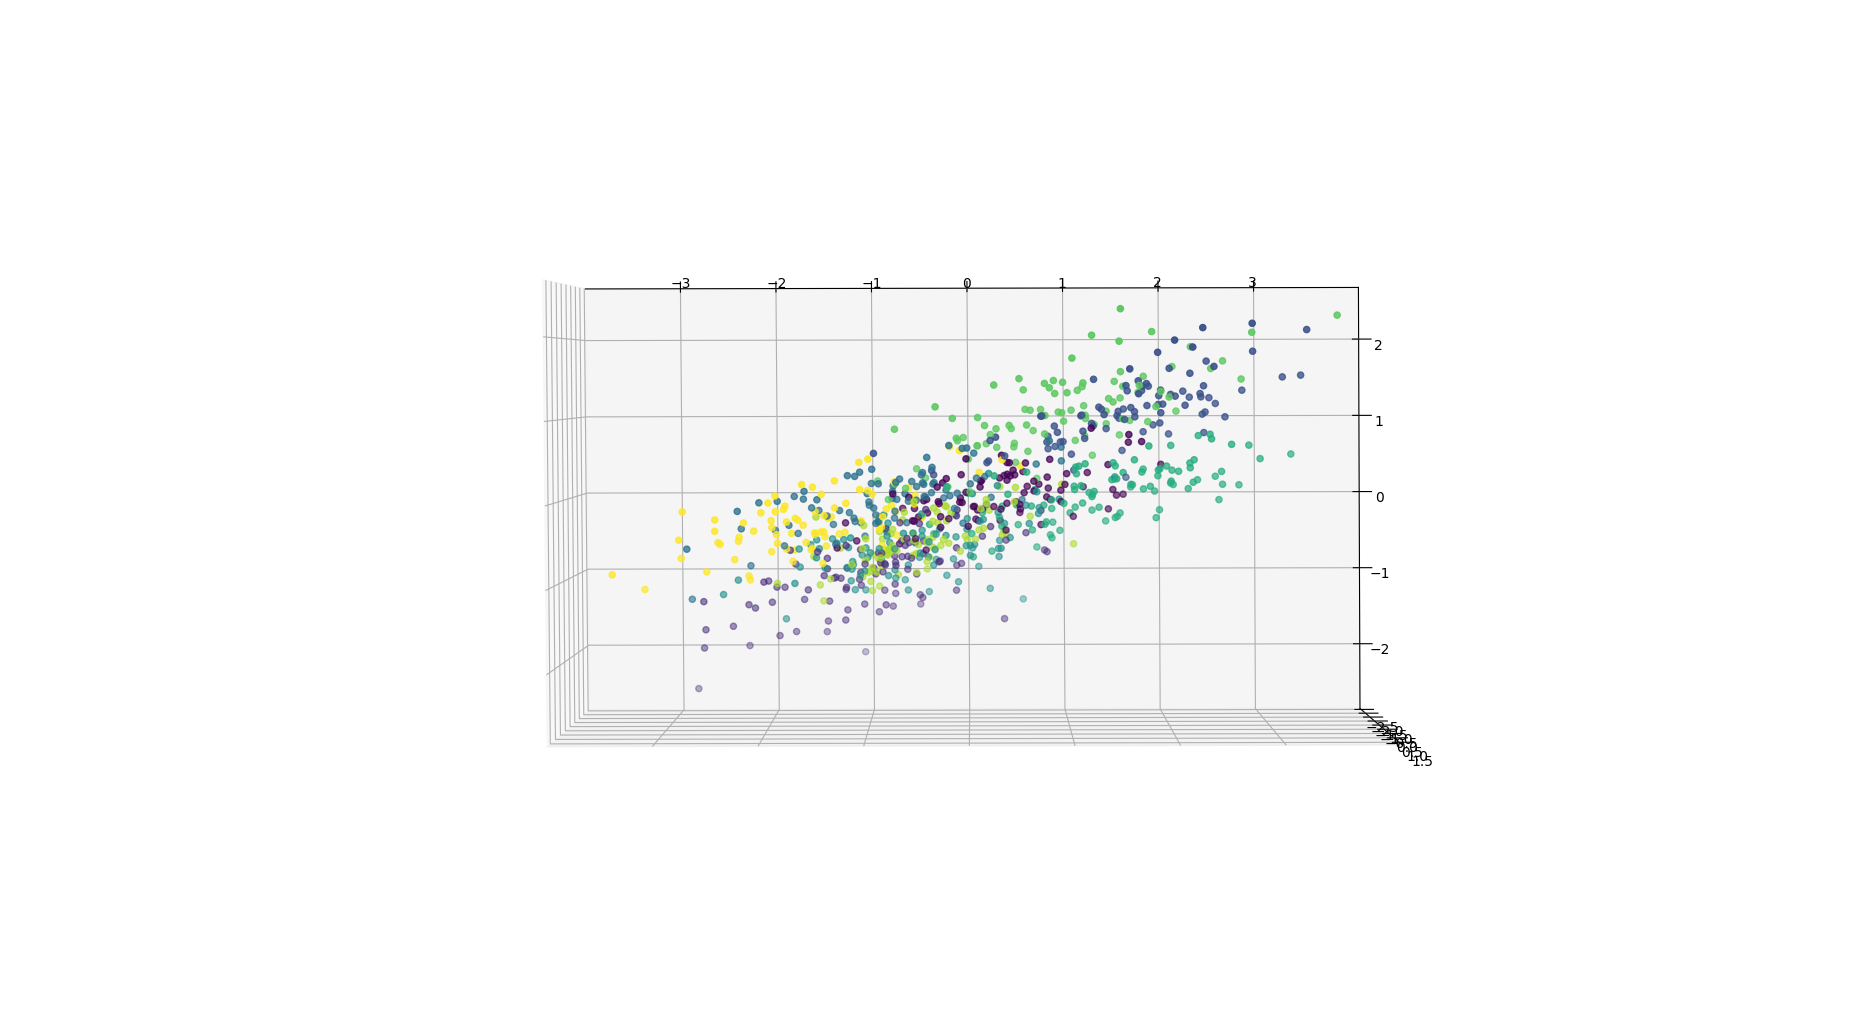
\includegraphics[width=1\linewidth, scale=1]{../img/ej1/sanger_corrida_200_9/sanger_9salida_200ep_testing_dim789_3.png}
  \caption{Sanger - 9 dimensiones - 200 épocas - Coordenadas 789}
  \label{fig:sub1}
\end{subfigure}%
\begin{subfigure}{.5\textwidth}
  \centering
  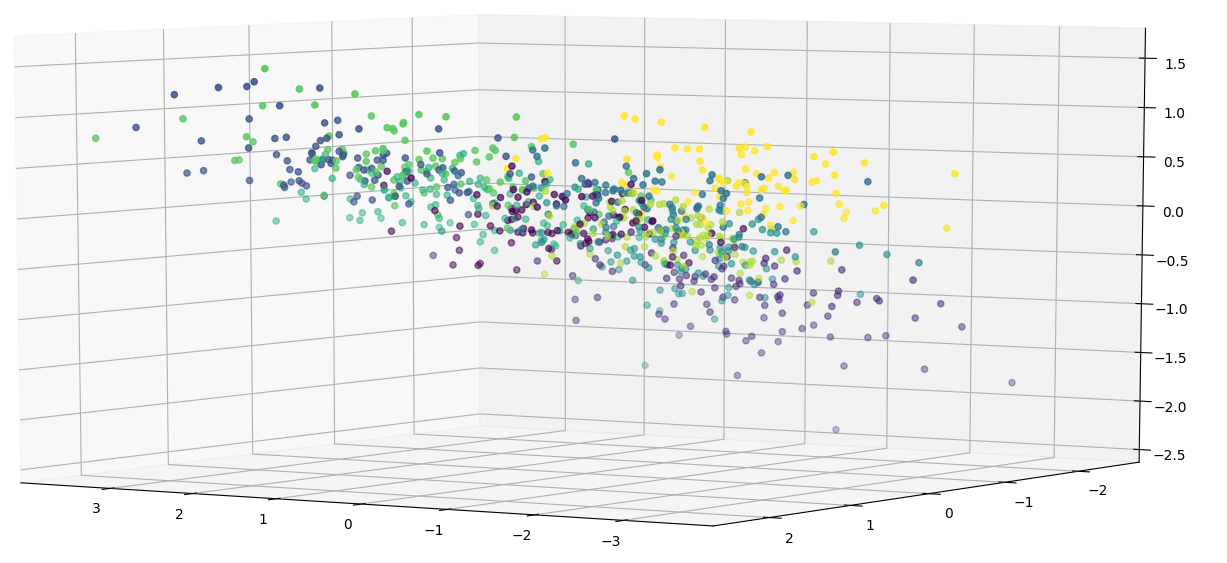
\includegraphics[width=1\linewidth, scale=1]{../img/ej1/sanger_corrida_200_9/sanger_9salida_200ep_testing_dim789_4.png}
  \caption{Sanger - 9 dimensiones - 200 épocas - Coordenadas 789}
  \label{fig:sub2}
\end{subfigure}
\end{figure}

En estas últimas se nota menos precisión en los clusters y mayor solapamiento. Sin embargo, considerado lo observado con Sanger en las primeras 3 coordenadas, éstos son los mejores
resultados que obtuvimos en todo el ejercicio 1. En el caso de esta regla, la ampliación a 9 dimensiones mostró una diferencia notable en la calidad de la solución.

\newpage
\subsection{Ejercicio 2 - Mapeo de características}

Para el segundo ejercicio, los experimentos consistieron en variar la cantidad de neuronas del mapa que podían ser activadas, en conjunto con la cantidad de épocas y la división de las mismas en ordenamiento y convergencia. Intentamos variar estos factores y observar diferencias en los gráficos de estilo mapa de calor generados en base a las categorías que activaron en mayor medida a cada una de las neuronas del mapa.

Comenzamos realizando clasificaciones con 200 épocas como el primer ejercicio, pero, si bien se pudieron apreciar algunos agrupamientos, no era lo esperado. Dado que además vimos que corría mucho más rápido que en el primer ejercicio, decidimos además subir las épocas a 1000 como se propone en lo visto en clase. Allí observamos una clasificación mejor, con agrupamientos bien definidos.

Estas pruebas fueron hechas tanto para el mapeo de los documentos directamente (donde cada neurona del mapa tiene 850 vectores de entrada), y para las 3 y 9 componentes principales que se obtienen de las redes generadas en el primer ejercicio. Para estos dos últimos casos, utilizaremos las redes generadas con el algoritmo de Sanger, dado que fue el que nos devolvió los mejores resultados.

Finalmente, comparamos los resultados obtenidos entre las 3 opciones para dar nuestra visión de cual funcionó mejor en base a nuestros experimentos.

\subsubsection{Mapeo de documentos con 850 atributos}

En primera instancia, planteamos un experimento utilizando 200 épocas, lo cual no produjo buenos resultados como mencionamos anteriormente. En consecuencia, aumentamos las épocas a 1000 como sugerencia de lo visto en clase. Decidimos tomar un mapa de neuronas de 10 x 10 como primera prueba. Nos pareció un buen número para empezar para darle oportunidad a cada neurona de que sea activada por más de un documento (810 documentos de entrenamiento sobre 100 neuronas del mapa). 

\begin{figure}[h]
  \begin{center}
    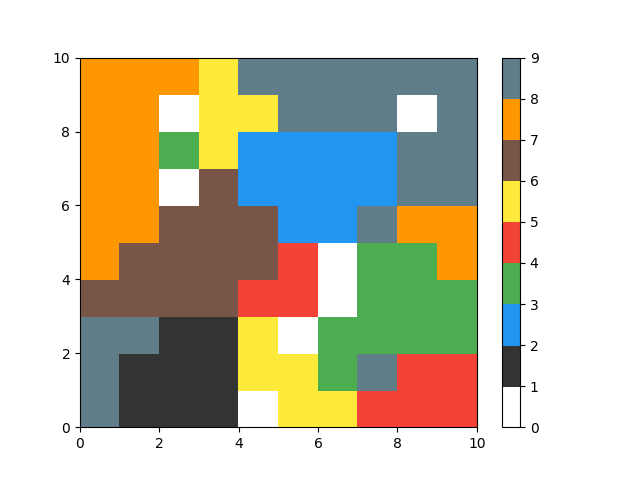
\includegraphics[scale=0.4]{../img/map_1000ep_850en.png}
  \caption{Mapa 10x10 - 850 ejes x neurona - 1000 épocas - Sigma 5 - Entrenamiento}
  \end{center}
\end{figure}

Si bien hay un idea de agrupamiento no es lo que esperábamos, por lo cual decidimos variar el parámetro T1 del cálculo del sigma inicial para que la función logaritmo del sigma que nosotros pasamos por parámetro le aplique logaritmo en base 2 en vez de logaritmo natural. Luego, volvimos a correr el experimento y obtuvimos mejores resultados.

\begin{figure}[h]
  \begin{center}
    \includegraphics[scale=0.4]{../img/map_1000ep_850en.png}
  \caption{Mapa 10x10 - 850 ejes x neurona - 1000 épocas - Sigma 5 - Entrenamiento}
  \end{center}
\end{figure}

Sin embargo, encontramos muy extraño que haya tantos blancos en el mapa, que significa que esas neuronas que están blancas no fueron activadas por ningún documento cuando realizamos la última pasada de los documentos sobre la red entrenada para armar el mapa. Esto nos desconcertó de si era correcto o no, con lo cual recurrimos a consultarlo con los profesores, lo que nos permitió entender que esto no debería suceder y que las posibles causas podían ser que nuestro mapa era demasiado grande, o que teníamos algún problema en la función de vecindad y/o las fases de ordenamiento y convergencia y/o nuestro código en sí.

Luego de revisar nuestra implementación, descubrimos que las fases de ordenamiento y convergencia no estaban muy bien definidas y que durante todas las épocas tanto el sigma como el eta no dejaban de ser \textit{enfriados}. Es por eso que decidimos plantear que de las 1000 épocas, dos tercios de las mismas sean de ordenamiento y el resto de convergencia. Además, decidimos achicar el área de nuestro mapa de neuronas de 10x10 a 8x8 y volvimos a correr el experimento.

\newpage
\section{Soluciones Óptimas Propuestas}

% Siguiendo las distintas conclusiones que fuimos formando a través de los experimentos, generamos una solución óptima para cada ejercicio del TP. Estas soluciones se encuentran codificadas en \textbf{solucion\_ej1.json} y \textbf{solucion\_ej2.json}.

% \subsection{Ejercicio 1}
% La solución del ejercicio 1 fue generada con los siguientes parámetros:

% \texttt{\$python script.py 1 -ep=250 -capas=10,10 -eta=0.05 -estop=0.1}

% La solución generó muy buenos resultados, obteniendo 94\% de efectividad con respecto a su dataset de testing.
% Con respecto al error final, así fue su evolución:

% \begin{figure}[h]
%   \begin{center}
%   \includegraphics[scale=0.50]{graficos/solucion_ej1.png}
%   \caption{Evolución del error a través del entrenamiento para la solución 1}
%   \end{center}
% \end{figure}

% Notamos que encontró valores muy bajos de error, con una curva bastante pronunciada a partir de la época 50. Observamos que el early stopping efectivamente entró en efecto, ya que cortó la ejecución antes de llegar al límite de épocas.\\

% En caso de querer cargar y probar esta red, ejecutar:

% \texttt{\$python script.py 1 -file=F -rda=solucion\_ej1.json -te=100 }

% donde \texttt{F} debe ser el path al archivo CSV que contenga el dataset seleccionado. El parámetro $te=100$ implica que se le ordena a la red predecir todos los resultados del dataset como testing y calcular su tasa de aciertos.

% \subsection{Ejercicio 2}
% La solución del ejercicio 2 fue generada con los siguientes parámetros:

% \texttt{\$python script.py 2 -ep=250 -capas=7 -estop=0.05}

% La solución generó resultados decentes, obteniendo 74\% de efectividad con respecto a su dataset de testing.\\
% Se nota una eficiencia menor a la de la solución del ejercicio 1.
% En la última figura podemos ver la evolución de las épocas y el error:

% \begin{figure}[h]
%   \begin{center}
%   \includegraphics[scale=0.50]{graficos/solucion_ej2.png}
%   \caption{Evolución del error a través del entrenamiento para la solución 2}
%   \end{center}
% \end{figure}

% \newpage

% Notamos en este caso un descenso más lento del error y un estancamiento final en la curva. No se llegó a aplicar la cláusula del early stopping.


% En caso de querer cargar y probar esta red, ejecutar:

% \texttt{\$python script.py 2 -file=F -rda=solucion\_ej2.json -te=100 }

% donde \texttt{F} debe ser el path al archivo CSV que contenga el dataset seleccionado.

% \newpage
\section{Conclusión}

% Como conclusión podemos ver que los distintos ejercicios y sus características obtuvieron diferentes resultados en los experimentos realizados.\\

% Notamos en ellos algunos fenómenos. En primer lugar, parecería que la cantidad óptima de neuronas en cada capa se acerca a la cantidad de atributos a procesar por la red. Esto se pudo observar en el experimento de cantidad de neuronas para cada ejercicios.\\
% En segundo lugar, apreciamos distintos efectos en la cantidad de épocas necesarias para llegar a buenos resultados. Cada ejercicio necesitó una cantidad diferente y muchos de los parámetros afectaron dicha cantidad, aumentándola ampliamente en varios casos.\\

% Algunos parámetros que pensamos que tendrían mayor efecto en los resultados fueron los de distribución de los pesos, momentum y en el caso del ejercicio 2, cantidad de capas. Nos sorprendió que finalmente la solución óptima no utilizara más estos factores.\\

% Aprendimos que parámetros como el early stopping, que de antemano parecía que si o si debería estar en nuestra solución, no nos dió resultados lo suficiente buenos 
% como para considerarlo como algo obligatorio a la hora de entrenar la red. Quizás esto fue porque la cantidad de épocas de nuestro entrenamiento no era la suficiente 
% como vimos anteriormente, y este relacionado también con que nuestro conjunto de datos es acotado, nuestra red pequeña y no se necesitan tantas épocas para entrenar.

% Vimos también que los parámetros adaptativos, como el learning rate, mejoran considerablemente soluciones como el entrenamiento batch o mini batch. Incluso, en el 
% entrenamiento batch, se puede llegar a conseguir una soluciones muy buenas si las épocas son suficientes con learning rate adaptativo.

% Finalmente observamos la naturaleza práctica de este tipo de problemas, en la cual muchos de las decisiones responden a experimentación y pruebas y no tanto a fundamentos teóricos o conceptuales.

	\newpage
	\section{Anexo - Código}
Incluimos aquí el código python de la aplicación. La explicación del contenido de cada archivo puede encontrarse en la introducción del informe.

\subsection{script.py}

\begin{changemargin}{-2.0cm}{-1.5cm} 
\begin{verbatim}

# -*- coding: utf-8 -*-
import csv
import random
import numpy as np
import matplotlib.pyplot as plt
from matplotlib import colors
from mpl_toolkits.mplot3d import Axes3D
import self_organized_map as som
import parameters as params
import encoder as encoder
import time

######### PARSEO DE PARAMETROS ##############

filepath, eta, epochs, regla, dimensiones, red_desde_archivo, 
  red_hacia_archivo, red_ej1 = params.iniciar()

######### PARSEO DE DATOS ##############

f = open('tp2_training_dataset.csv', 'rb')
reader = csv.reader(f)
categorias_verificacion = []
atributos = []

for row in reader:
    categoria = float(row.pop(0))
    categorias_verificacion.append(categoria)
    atributos.append([float(x) for x in row])

f.close()

######## MEDIA 0 POR COLUMNA ##############

matrix = np.array(atributos)
column_means = np.mean(matrix, axis=0)

for i, mean in enumerate(column_means):
    for j, _ in enumerate(matrix):
        matrix[j][i] = matrix[j][i] - mean

# Aca ordenamos al azar los documentos y sus categorias
# de manera de siempre agarrar distintos conjuntos de train y validation
rnd_state = np.random.get_state()
np.random.shuffle(matrix)
np.random.set_state(rnd_state)
np.random.shuffle(categorias_verificacion)


dataset_train = matrix[:int(len(matrix) * 0.9)]
dataset_validation = matrix[int(len(matrix) * 0.9):]

######## TRAINING ##############

# Si se va a ejecutar reduciendo dimensiones con redes del ej1, tomar nentrada del tam apropiado
if red_ej1 is not None:
    n_entrada = dimensiones
else:
    n_entrada = len(atributos[0])

map_size = 7
sigma = 7
longer_width = 0

if red_desde_archivo:
    SOM = encoder.from_json(red_desde_archivo, 2)
else:
    SOM = som.SelfOrganizedMap(n_entrada, map_size, offset_width_map=longer_width)

# Si proveo red del ej1 para redurcir, entonces no tomar los documentos enteros sino
# Reducir dimensionalidad utilizando dicha red
if red_ej1 is not None:
    coordenadas = SOM.translate_documentos_to_coordenadas(dataset_train, red_ej1)
    coordenadas_validation = SOM.translate_documentos_to_coordenadas(dataset_validation, red_ej1)

    # Si la red es nueva, entrenarla
    if red_desde_archivo is None:
        start = time.time()
        SOM.train_con_documentos(coordenadas, sigma=sigma, epochs=epochs)
        end = time.time()
        print 'Tiempo de corrida: '+ str(end - start)

    resultados = SOM.predict(coordenadas, categorias_verificacion)

# Si no hay red ej1, usar dataset default
else:
    # Si la red es nueva, entrenarla
    if red_desde_archivo is None:
        start = time.time()
        SOM.train_con_documentos(dataset_train, sigma=sigma, epochs=epochs)
        end = time.time()
        print 'Tiempo de corrida: '+ str(end - start)

    resultados = SOM.predict(dataset_train, categorias_verificacion)


########## OUTPUT A JSON ##############
if red_hacia_archivo:
    encoder.to_json(red_hacia_archivo, SOM, 2)

########## OBTENCION COORDENADAS ##############

cmap = colors.ListedColormap(
    [
        'white', 
        (51.0/256.0, 51.0/256.0, 51.0/256.0, 1), 
        (33.0/256.0, 150.0/256.0, 243.0/256.0, 1),
        (76.0/256.0, 175.0/256.0, 80.0/256.0, 1),
        (244.0/256.0, 67.0/256.0, 54.0/256.0, 1),
        (255.0/256.0, 235.0/256.0, 59.0/256.0, 1),
        (121.0/256.0, 85.0/256.0, 72.0/256.0, 1),
        (255.0/256.0, 152.0/256.0, 0.0/256.0, 1),
        (156.0/256.0, 39.0/256.0, 176.0/256.0, 1),
        (96.0/256.0, 125.0/256.0, 139.0/256.0, 1),
        (63.0/256.0, 81.0/256.0, 181.0/256.0, 1)
    ]
)
bounds = range(11)
norm = colors.BoundaryNorm(bounds, cmap.N)

column_labels = range(map_size)
row_labels = range(map_size+longer_width)
heatmap = plt.pcolor(np.array(resultados), cmap=cmap, norm=norm)
heatmap.axes.set_xticklabels = column_labels
heatmap.axes.set_yticklabels = row_labels
m = plt.colorbar(heatmap, ticks=range(11))

plt.show()

######### CALCULO DEL ERROR CON VALIDACION ###########

if red_ej1 is not None:
    errores_x_categoria = SOM.validation_error(coordenadas_validation, resultados, 
      categorias_verificacion, int(len(matrix) * 0.9))
else:
    errores_x_categoria = SOM.validation_error(dataset_validation, resultados, 
      categorias_verificacion, int(len(matrix) * 0.9))

fig = plt.figure()
chart_bar = fig.add_subplot(111)

y = [q[1] for q in errores_x_categoria]
x = [q[0] for q in errores_x_categoria]
width = 1/1.5
chart_bar.bar(x, y, width, color=(63.0/256.0, 81.0/256.0, 181.0/256.0, 1))

plt.show()
\end{verbatim}
\end{changemargin}

\newpage
\subsection{network.py}

\begin{changemargin}{-2.0cm}{-1.5cm} 
\begin{verbatim}
# -*- coding: utf-8 -*-
import numpy as np

class UnsupervisedLearningNetwork(object):

    def __init__(self, n_entrada=1, n_salida=3, basic_init_pesos=None):
        self.pesos_red = list()

        # Para cargar redes armadas con pesos ya entrenados
        if basic_init_pesos is not None:
            self.pesos_red = basic_init_pesos
        else:
            for _ in range(n_salida):
                self.pesos_red.append({'pesos': np.random.uniform(-0.1, 0.1, n_entrada)})

    def train_ej1(self, dataset, eta=0.01, epochs=10, algoritmo="sanger"):

        # for X en D:
        #     Y = X . W
        #     for j en [1..M]:
        #         for i en [1..N]:
        #             X~_i = 0
        #             for k en [1..Q]
        #                 X~_i += Y_k . W_ik
        #             DeltaW_ij = eta . (X_i - X~_i) . Y_j
        #     W += DeltaW

        for ep in range(epochs):
            
            for _, documento in enumerate(dataset):
                y = list()

                # Recorro las neuronas de salida 2 veces porque necesito tener
                # calculadas las salidas de las mismas para hacer Oja
                for n_neurona in range(len(self.pesos_red)):
                    salida_neurona = np.dot(documento, self.pesos_red[n_neurona]['pesos'])
                    y.append(salida_neurona)

                # Para todas las neuronas de salida, se actualizan los pesos de
                # las 850 entradas para cada documento
                for n_neurona in range(len(self.pesos_red)):           
                    delta_w = list()
                    
                    for i, atributo in enumerate(documento):
                        x = 0

                        # Las salidas utilizadas para actualizar los pesos dependen
                        # de si se usa Oja o Sanger
                        for k in range(self.calcular_intervalo(algoritmo, n_neurona)):
                            x += y[k] * self.pesos_red[k]['pesos'][i]

                        delta_w.append(eta * (atributo - x) * salida_neurona)

                    # Actualizacion de los pesos
                    self.pesos_red[n_neurona]['pesos'] = 
                      np.sum([self.pesos_red[n_neurona]['pesos'], delta_w], axis=0)
            
            print 'Finalizada epoca '+str(ep)

        return self

    def predict_coordenadas_ej1(self, documento):
        coordenadas = list()

        for n_neurona in range(len(self.pesos_red)):
            salida_neurona = np.dot(documento, self.pesos_red[n_neurona]['pesos'])
            coordenadas.append(salida_neurona)

        return coordenadas

    def calcular_intervalo(self, algoritmo, neurona_actual):
        if algoritmo == "hebb":
            return 0
        
        if algoritmo == "oja1":
            return 1

        if algoritmo == "oja":
            return len(self.pesos_red)
        
        if algoritmo == "sanger":
            return neurona_actual+1

\end{verbatim}
\end{changemargin}

\newpage
\subsection{script\_map.py}

\begin{changemargin}{-2.0cm}{-1.5cm} 
\begin{verbatim}
# -*- coding: utf-8 -*-
import csv
import random
import numpy as np
import matplotlib.pyplot as plt
from matplotlib import colors
from mpl_toolkits.mplot3d import Axes3D
import self_organized_map as som
import parameters as params
import encoder as encoder
import time

######### PARSEO DE PARAMETROS ##############

filepath, eta, epochs, regla, dimensiones, red_desde_archivo, red_hacia_archivo, red_ej1 = 
  params.iniciar()

######### PARSEO DE DATOS ##############

f = open('tp2_training_dataset.csv', 'rb')
reader = csv.reader(f)
categorias_verificacion = []
atributos = []

for row in reader:
    categoria = float(row.pop(0))
    categorias_verificacion.append(categoria)
    atributos.append([float(x) for x in row])

f.close()

######## MEDIA 0 POR COLUMNA ##############

matrix = np.array(atributos)
column_means = np.mean(matrix, axis=0)

for i, mean in enumerate(column_means):
    for j, _ in enumerate(matrix):
        matrix[j][i] = matrix[j][i] - mean

# Aca ordenamos al azar los documentos y sus categorias
# de manera de siempre agarrar distintos conjuntos de train y validation
rnd_state = np.random.get_state()
np.random.shuffle(matrix)
np.random.set_state(rnd_state)
np.random.shuffle(categorias_verificacion)


dataset_train = matrix[:int(len(matrix) * 0.9)]
dataset_validation = matrix[int(len(matrix) * 0.9):]

######## TRAINING ##############

# Si se va a ejecutar reduciendo dimensiones con redes del ej1, tomar nentrada del tam apropiado
if red_ej1 is not None:
    n_entrada = dimensiones
else:
    n_entrada = len(atributos[0])

map_size = 7
sigma = 7
longer_width = 0

if red_desde_archivo:
    SOM = encoder.from_json(red_desde_archivo, 2)
else:
    SOM = som.SelfOrganizedMap(n_entrada, map_size, offset_width_map=longer_width)

# Si proveo red del ej1 para redurcir, entonces no tomar los documentos enteros sino
# Reducir dimensionalidad utilizando dicha red
if red_ej1 is not None:
    coordenadas = SOM.translate_documentos_to_coordenadas(dataset_train, red_ej1)
    coordenadas_validation = 
      SOM.translate_documentos_to_coordenadas(dataset_validation, red_ej1)

    # Si la red es nueva, entrenarla
    if red_desde_archivo is None:
        start = time.time()
        SOM.train_con_documentos(coordenadas, sigma=sigma, epochs=epochs)
        end = time.time()
        print 'Tiempo de corrida: '+ str(end - start)

    resultados = SOM.predict(coordenadas, categorias_verificacion)

# Si no hay red ej1, usar dataset default
else:
    # Si la red es nueva, entrenarla
    if red_desde_archivo is None:
        start = time.time()
        SOM.train_con_documentos(dataset_train, sigma=sigma, epochs=epochs)
        end = time.time()
        print 'Tiempo de corrida: '+ str(end - start)

    resultados = SOM.predict(dataset_train, categorias_verificacion)


########## OUTPUT A JSON ##############
if red_hacia_archivo:
    encoder.to_json(red_hacia_archivo, SOM, 2)

########## OBTENCION COORDENADAS ##############

cmap = colors.ListedColormap(
    [
        'white', 
        (51.0/256.0, 51.0/256.0, 51.0/256.0, 1), 
        (33.0/256.0, 150.0/256.0, 243.0/256.0, 1),
        (76.0/256.0, 175.0/256.0, 80.0/256.0, 1),
        (244.0/256.0, 67.0/256.0, 54.0/256.0, 1),
        (255.0/256.0, 235.0/256.0, 59.0/256.0, 1),
        (121.0/256.0, 85.0/256.0, 72.0/256.0, 1),
        (255.0/256.0, 152.0/256.0, 0.0/256.0, 1),
        (156.0/256.0, 39.0/256.0, 176.0/256.0, 1),
        (96.0/256.0, 125.0/256.0, 139.0/256.0, 1),
        (63.0/256.0, 81.0/256.0, 181.0/256.0, 1)
    ]
)
bounds = range(11)
norm = colors.BoundaryNorm(bounds, cmap.N)

column_labels = range(map_size)
row_labels = range(map_size+longer_width)
heatmap = plt.pcolor(np.array(resultados), cmap=cmap, norm=norm)
heatmap.axes.set_xticklabels = column_labels
heatmap.axes.set_yticklabels = row_labels
m = plt.colorbar(heatmap, ticks=range(11))

plt.show()

######### CALCULO DEL ERROR CON VALIDACION ###########

if red_ej1 is not None:
    errores_x_categoria = SOM.validation_error(coordenadas_validation, 
      resultados, categorias_verificacion, int(len(matrix) * 0.9))
else:
    errores_x_categoria = SOM.validation_error(dataset_validation, 
      resultados, categorias_verificacion, int(len(matrix) * 0.9))

fig = plt.figure()
chart_bar = fig.add_subplot(111)

y = [q[1] for q in errores_x_categoria]
x = [q[0] for q in errores_x_categoria]
width = 1/1.5
chart_bar.bar(x, y, width, color=(63.0/256.0, 81.0/256.0, 181.0/256.0, 1))

plt.show()

\end{verbatim}
\end{changemargin}

\newpage
\subsection{self\_organized\_map.py}

\begin{changemargin}{-2.0cm}{-1.5cm} 
\begin{verbatim}
# -*- coding: utf-8 -*-
from math import e, log
import numpy as np
import encoder as encoder

class SelfOrganizedMap(object):

    def __init__(self, n_entrada = 1, map_size = 7, basic_init_pesos=None, offset_width_map=0):

        # Para cargar redes armadas con pesos ya entrenados
        if basic_init_pesos is not None:
            self.map = basic_init_pesos
        else:
            matrix = []

            for _ in range(map_size):
                row = []
                for _ in range(map_size+offset_width_map):
                    row.append({'pesos': np.random.uniform(-0.1, 0.1, n_entrada)})

                matrix.append(row)

            self.map = matrix

    def translate_documentos_to_coordenadas(self, documentos, sanger_network_file):
        ppn = encoder.from_json(sanger_network_file, 1)
        coordenadas = []

        for documento in documentos:
            coordenadas.append(ppn.predict_coordenadas_ej1(documento))

        return coordenadas

    def train_con_documentos(self, documentos, sigma=5, eta=0.1, epochs=10):
        iteration = 0.0
        sigma_0 = sigma
        eta_0 = eta
        t1_sigma = float(epochs) / float(log(sigma_0, 2))
        t2_eta = float(epochs)

        for ep in range(epochs):
            
            for _, documento in enumerate(documentos):
                winner_index = []
                min_distancia = float('inf')

                # Calculo todas las salidas de las neuronas de mi mapa
                for i, row in enumerate(self.map):
                    for j, _ in enumerate(row):
                        distancia = self.distancia_geometrica(documento, self.map[i][j]['pesos'])

                        # Voy calculando cual es la neurona ganadora
                        if distancia < min_distancia:
                            min_distancia = distancia
                            winner_index = np.array([i, j])
            
                for i, row in enumerate(self.map):
                    for j, _ in enumerate(row):

                        # Actualizacion de los pesos de las
                        # neuronas con la funcion de vecindad
                        h = self.funcion_vecindad(np.array([i, j]), winner_index, sigma)

                        self.map[i][j]['pesos'] += 
                          eta * h * np.subtract(documento, self.map[i][j]['pesos'])
            
            if iteration < (epochs * 3 / 4):
                sigma, eta = self.cooling(iteration, sigma_0, t1_sigma, eta_0, t2_eta)
            
            iteration += 1

            print 'Finalizada epoca '+str(ep)

        return self

    def predict(self, documentos, categorias):
        resultados = []

        for r1, row in enumerate(self.map):
            resultados.append([])

            for _ in enumerate(row):
                resultados[r1].append([])

        for k, documento in enumerate(documentos):
            winner_index = []
            min_distancia = float('inf')

            # Calculo todas las salidas de las neuronas de mi mapa
            for i, row in enumerate(self.map):
                for j, _ in enumerate(row):
                    distancia = self.distancia_geometrica(documento, self.map[i][j]['pesos'])

                    # Voy calculando cual es la neurona ganadora
                    if distancia < min_distancia:
                        min_distancia = distancia
                        winner_index = np.array([i, j])

            resultados[winner_index[0]][winner_index[1]].append(categorias[k])

        return self.determinar_categoria_ganadora(resultados)

    def validation_error(self, docs_validation, resultados_training, categorias, offset=0):
        error_x_categoria = [(x+1, 0) for x in range(9)]

        for k, documento in enumerate(docs_validation):
            winner_index = []
            min_distancia = float('inf')

            # Calculo todas las salidas de las neuronas de mi mapa
            for i, row in enumerate(self.map):
                for j, _ in enumerate(row):
                    distancia = self.distancia_geometrica(documento, self.map[i][j]['pesos'])

                    # Voy calculando cual es la neurona ganadora
                    if distancia < min_distancia:
                        min_distancia = distancia
                        winner_index = np.array([i, j])

            categoria_training = resultados_training[winner_index[0]][winner_index[1]]

            if categoria_training != categorias[k+int(offset)]:
                error_x_categoria[categoria_training-1] = 
                  (categoria_training, error_x_categoria[categoria_training-1][1]+1)

        return error_x_categoria

    def print_nice(self, data):
        for row in data:
            print row

    def determinar_categoria_ganadora(self, neurona_categorias):
        mas_comunes = []

        for i, neurona in enumerate(neurona_categorias):
            mas_comunes.append([])
            
            for _, categorias in enumerate(neurona):
                mas_comunes[i].append(self.mas_comun(categorias))

        return mas_comunes
                
    def mas_comun(self, categorias):
        if len(categorias) == 0:
            return 0

        return int(max(set(categorias), key=categorias.count))

    def funcion_vecindad(self, neurona, ganadora, sigma):
        return e**(-(self.distancia_geometrica(neurona, ganadora)**2 / 2*(sigma**2)))

    def distancia_geometrica(self, rj, ri):
        return float(np.linalg.norm(rj-ri))

    def cooling(self, iteration_number, sigma_0, t1_sigma, eta_0, t2_eta):
        new_sigma = sigma_0 * (e**(-(iteration_number / t1_sigma)))
        new_eta = eta_0 * (e**(-(iteration_number / t2_eta)))

        return new_sigma, new_eta
\end{verbatim}
\end{changemargin}

\newpage
\subsection{encoder.py}

\begin{changemargin}{-2.0cm}{-1.5cm} 
\begin{verbatim}
# -*- coding: utf-8 -*-
import network as ppn
import self_organized_map as som
import numpy as np
import io, json
from json import JSONEncoder

def to_json(filepath, red, numero_ejercicio):
    with io.open(filepath, 'w', encoding='utf-8') as f:

        if numero_ejercicio == 1:
            pesos = red.pesos_red

            for pesos_capa in pesos:
                pesos_capa['pesos'] = pesos_capa['pesos'].tolist()

            f.write(unicode(json.dumps(pesos, ensure_ascii=False)))
        else:
            pesos = red.map

            for i, row in enumerate(pesos):
                for j, subrow in enumerate(row):
                    pesos[i][j]['pesos'] = pesos[i][j]['pesos'].tolist()

            f.write(unicode(json.dumps(pesos, ensure_ascii=False)))

def from_json(filepath, numero_ejercicio):
    with open(filepath, 'r') as content_file:
        content = content_file.read()
        pesos = json.loads(content)

        if numero_ejercicio == 1:
            for pesos_capa in pesos:
                pesos_capa['pesos'] = np.array(pesos_capa['pesos'])

            return ppn.UnsupervisedLearningNetwork(basic_init_pesos=pesos)

        else:
            for i, row in enumerate(pesos):
                for j, subrow in enumerate(row):
                    pesos[i][j]['pesos'] = np.array(pesos[i][j]['pesos'])

            return som.SelfOrganizedMap(basic_init_pesos=pesos)

\end{verbatim}
\end{changemargin}|
	\newpage
\end{document}

